%==============================================================================
% tento soubor pouzijte jako zaklad
% this file should be used as a base for the thesis
% Autoři / Authors: 2008 Michal Bidlo, 2019 Jaroslav Dytrych
% Kontakt pro dotazy a připomínky: sablona@fit.vutbr.cz
% Contact for questions and comments: sablona@fit.vutbr.cz
%==============================================================================
% kodovani: UTF-8 (zmena prikazem iconv, recode nebo cstocs)
% encoding: UTF-8 (you can change it by command iconv, recode or cstocs)
%------------------------------------------------------------------------------
% zpracování / processing: make, make pdf, make clean
%==============================================================================
% Soubory, které je nutné upravit nebo smazat: / Files which have to be edited or deleted:
%   xfurda00_2020-20-literatura-bibliography.bib - literatura / bibliography
%   xfurda00_2020-01-kapitoly-chapters.tex - obsah práce / the thesis content
%   xfurda00_2020-01-kapitoly-chapters-en.tex - obsah práce v angličtině / the thesis content in English
%   xfurda00_2020-30-prilohy-appendices.tex - přílohy / appendices
%   xfurda00_2020-30-prilohy-appendices-en.tex - přílohy v angličtině / appendices in English
%==============================================================================
%\documentclass[]{fitthesis} % bez zadání - pro začátek práce, aby nebyl problém s překladem
%\documentclass[english]{fitthesis} % without assignment - for the work start to avoid compilation problem
\documentclass[zadani]{fitthesis} % odevzdani do wisu a/nebo tisk s barevnými odkazy - odkazy jsou barevné
%\documentclass[english,zadani]{fitthesis} % for submission to the IS FIT and/or print with color links - links are color
%\documentclass[zadani,print]{fitthesis} % pro černobílý tisk - odkazy jsou černé
%\documentclass[english,zadani,print]{fitthesis} % for the black and white print - links are black
%\documentclass[zadani,cprint]{fitthesis} % pro barevný tisk - odkazy jsou černé, znak VUT barevný
%\documentclass[english,zadani,cprint]{fitthesis} % for the print - links are black, logo is color
% * Je-li práce psaná v anglickém jazyce, je zapotřebí u třídy použít 
%   parametr english následovně:
%   If thesis is written in English, it is necessary to use 
%   parameter english as follows:
%      \documentclass[english]{fitthesis}
% * Je-li práce psaná ve slovenském jazyce, je zapotřebí u třídy použít 
%   parametr slovak následovně:
%   If the work is written in the Slovak language, it is necessary 
%   to use parameter slovak as follows:
%      \documentclass[slovak]{fitthesis}
% * Je-li práce psaná v anglickém jazyce se slovenským abstraktem apod., 
%   je zapotřebí u třídy použít parametry english a enslovak následovně:
%   If the work is written in English with the Slovak abstract, etc., 
%   it is necessary to use parameters english and enslovak as follows:
%      \documentclass[english,enslovak]{fitthesis}

% Základní balíčky jsou dole v souboru šablony fitthesis.cls
% Basic packages are at the bottom of template file fitthesis.cls
% zde můžeme vložit vlastní balíčky / you can place own packages here

% Kompilace po částech (rychlejší, ale v náhledu nemusí být vše aktuální)
% Compilation piecewise (faster, but not all parts in preview will be up-to-date)
% \usepackage{subfiles}

% Nastavení cesty k obrázkům
% Setting of a path to the pictures
%\graphicspath{{obrazky-figures/}{./obrazky-figures/}}
%\graphicspath{{obrazky-figures/}{../obrazky-figures/}}

%---rm---------------
\renewcommand{\rmdefault}{lmr}%zavede Latin Modern Roman jako rm / set Latin Modern Roman as rm
%---sf---------------
\renewcommand{\sfdefault}{qhv}%zavede TeX Gyre Heros jako sf
%---tt------------
\renewcommand{\ttdefault}{lmtt}% zavede Latin Modern tt jako tt

% vypne funkci šablony, která automaticky nahrazuje uvozovky,
% aby nebyly prováděny nevhodné náhrady v popisech API apod.
% disables function of the template which replaces quotation marks
% to avoid unnecessary replacements in the API descriptions etc.
\csdoublequotesoff



\usepackage{url}


% =======================================================================
% balíček "hyperref" vytváří klikací odkazy v pdf, pokud tedy použijeme pdflatex
% problém je, že balíček hyperref musí být uveden jako poslední, takže nemůže
% být v šabloně
% "hyperref" package create clickable links in pdf if you are using pdflatex.
% Problem is that this package have to be introduced as the last one so it 
% can not be placed in the template file.
\ifWis
\ifx\pdfoutput\undefined % nejedeme pod pdflatexem / we are not using pdflatex
\else
  \usepackage{color}
  \usepackage[unicode,colorlinks,hyperindex,plainpages=false,pdftex]{hyperref}
  \definecolor{hrcolor-ref}{RGB}{223,52,30}
  \definecolor{hrcolor-cite}{HTML}{2F8F00}
  \definecolor{hrcolor-urls}{HTML}{092EAB}
  \hypersetup{
	linkcolor=hrcolor-ref,
	citecolor=hrcolor-cite,
	filecolor=magenta,
	urlcolor=hrcolor-urls
  }
  \def\pdfBorderAttrs{/Border [0 0 0] }  % bez okrajů kolem odkazů / without margins around links
  \pdfcompresslevel=9
\fi
\else % pro tisk budou odkazy, na které se dá klikat, černé / for the print clickable links will be black
\ifx\pdfoutput\undefined % nejedeme pod pdflatexem / we are not using pdflatex
\else
  \usepackage{color}
  \usepackage[unicode,colorlinks,hyperindex,plainpages=false,pdftex,urlcolor=black,linkcolor=black,citecolor=black]{hyperref}
  \definecolor{links}{rgb}{0,0,0}
  \definecolor{anchors}{rgb}{0,0,0}
  \def\AnchorColor{anchors}
  \def\LinkColor{links}
  \def\pdfBorderAttrs{/Border [0 0 0] } % bez okrajů kolem odkazů / without margins around links
  \pdfcompresslevel=9
\fi
\fi
% Řešení problému, kdy klikací odkazy na obrázky vedou za obrázek
% This solves the problems with links which leads after the picture
\usepackage[all]{hypcap}

% Informace o práci/projektu / Information about the thesis
%---------------------------------------------------------------------------
\projectinfo{
  %Prace / Thesis
  project={BP},            %typ práce BP/SP/DP/DR  / thesis type (SP = term project)
  year={2020},             % rok odevzdání / year of submission
  date=\today,             % datum odevzdání / submission date
  %Nazev prace / thesis title
  title.cs={Webový kanban},  % název práce v češtině či slovenštině (dle zadání) / thesis title in czech language (according to assignment)
  title.en={Web Kanban}, % název práce v angličtině / thesis title in english
  %title.length={14.5cm}, % nastavení délky bloku s titulkem pro úpravu zalomení řádku (lze definovat zde nebo níže) / setting the length of a block with a thesis title for adjusting a line break (can be defined here or below)
  %sectitle.length={14.5cm}, % nastavení délky bloku s druhým titulkem pro úpravu zalomení řádku (lze definovat zde nebo níže) / setting the length of a block with a second thesis title for adjusting a line break (can be defined here or below)
  %Autor / Author
  author.name={Jiří},   % jméno autora / author name
  author.surname={Furda},   % příjmení autora / author surname 
  %author.title.p={Bc.}, % titul před jménem (nepovinné) / title before the name (optional)
  %author.title.a={Ph.D.}, % titul za jménem (nepovinné) / title after the name (optional)
  %Ustav / Department
  department={UIFS}, % doplňte příslušnou zkratku dle ústavu na zadání: UPSY/UIFS/UITS/UPGM / fill in appropriate abbreviation of the department according to assignment: UPSY/UIFS/UITS/UPGM
  % Školitel / supervisor
  supervisor.name={Radek},   % jméno školitele / supervisor name 
  supervisor.surname={Burget},   % příjmení školitele / supervisor surname
  supervisor.title.p={Ing.},   %titul před jménem (nepovinné) / title before the name (optional)
  supervisor.title.a={Ph.D.},    %titul za jménem (nepovinné) / title after the name (optional)
  % Klíčová slova / keywords
  keywords.cs={Kanban, řízení projektů, agilní metodiky, web, Angular, ASP.NET, JavaScript, C\#}, % klíčová slova v českém či slovenském jazyce / keywords in czech or slovak language
  keywords.en={Kanban, project managment, agile methods, web, Angular, ASP.NET, JavaScript, C\#}, % klíčová slova v anglickém jazyce / keywords in english
  %keywords.en={Here, individual keywords separated by commas will be written in English.},
  % Abstrakt / Abstract
  abstract.cs={Tato bakalářská práce se zabývá vytvořením webové aplikace pro řízení projektů za pomocí agilní metodiky Kanban. Aplikace musí být implementovaná dle požadavků společnosti SEACOMP s.r.o., která ji bude využívat. Teoretická část práce se zaměřuje na problematiku projektového řízení a popisuje technologie použité při vývoji aplikace. Praktická část práce obsahuje popis návrhu aplikace a konkrétních částí její implementace. Výsledná aplikace byla otestována zaměstnanci společnosti a zhodnocena v~závěru práce.}, % abstrakt v českém či slovenském jazyce / abstract in czech or slovak language
  abstract.en={This bachelor thesis deals with the creation of a web application for project management using the agile methodology Kanban. The application must be implemented according to the requirements of SEACOMP s.r.o., which will use it. The theoretical part of the thesis focuses on the issue of project management and describes the technologies used in the development of the application. The practical part of the work contains a description of the application design and specific parts of its implementation. The resulting application was tested by the company's employees and evaluated at the end of the thesis.}, % abstrakt v anglickém jazyce / abstract in english
  %abstract.en={An abstract of the work in English will be written in this paragraph.},
  % Prohlášení (u anglicky psané práce anglicky, u slovensky psané práce slovensky) / Declaration (for thesis in english should be in english)
  declaration={Prohlašuji, že jsem tuto bakalářskou práci vypracoval samostatně pod vedením pana\linebreak Ing.~Radka Burgeta, Ph.D.
Další informace mi poskytl pan Ing.~Pavel Vyskočil.
Uvedl jsem všechny literární prameny a publikace, ze kterých jsem čerpal.},
  %declaration={I hereby declare that this Bachelor's thesis was prepared as an original work by the author under the supervision of Mr. X
% The supplementary information was provided by Mr. Y
% I have listed all the literary sources, publications and other sources, which were used during the preparation of this thesis.},
  % Poděkování (nepovinné, nejlépe v jazyce práce) / Acknowledgement (optional, ideally in the language of the thesis)
  acknowledgment={Děkuji mému vedoucímu panu Ing.~Radkovi Burgetovi, Ph.D. a konzultantovi panu Ing.~Pavlovi Vyskočilovi za odborné vedení a cenné rady během řešení této bakalářské práce. Dále bych chtěl poděkovat panu Mgr.~Davidu Bryšovi, za umožnění pracovat na firemním zadání diplomové práce a všem svým kolegům, kteří se zapojili do testování aplikace.},
  %acknowledgment={Here it is possible to express thanks to the supervisor and to the people which provided professional help
%(external submitter, consultant, etc.).},
  % Rozšířený abstrakt (cca 3 normostrany) - lze definovat zde nebo níže / Extended abstract (approximately 3 standard pages) - can be defined here or below
  %extendedabstract={Do tohoto odstavce bude zapsán rozšířený výtah (abstrakt) práce v českém (slovenském) jazyce.},
  %faculty={FIT}, % FIT/FEKT/FSI/FA/FCH/FP/FAST/FAVU/USI/DEF
  faculty.cs={Fakulta informačních technologií}, % Fakulta v češtině - pro využití této položky výše zvolte fakultu DEF / Faculty in Czech - for use of this entry select DEF above
  faculty.en={Faculty of Information Technology}, % Fakulta v angličtině - pro využití této položky výše zvolte fakultu DEF / Faculty in English - for use of this entry select DEF above
  department.cs={Ústav informačních systémů}, % Ústav v češtině - pro využití této položky výše zvolte ústav DEF nebo jej zakomentujte / Department in Czech - for use of this entry select DEF above or comment it out
  department.en={Department of Information Systems} % Ústav v angličtině - pro využití této položky výše zvolte ústav DEF nebo jej zakomentujte / Department in English - for use of this entry select DEF above or comment it out
}

% Rozšířený abstrakt (cca 3 normostrany) - lze definovat zde nebo výše / Extended abstract (approximately 3 standard pages) - can be defined here or above
%\extendedabstract{Do tohoto odstavce bude zapsán výtah (abstrakt) práce v českém (slovenském) jazyce.}

% nastavení délky bloku s titulkem pro úpravu zalomení řádku - lze definovat zde nebo výše / setting the length of a block with a thesis title for adjusting a line break - can be defined here or above
%\titlelength{14.5cm}
% nastavení délky bloku s druhým titulkem pro úpravu zalomení řádku - lze definovat zde nebo výše / setting the length of a block with a second thesis title for adjusting a line break - can be defined here or above
%\sectitlelength{14.5cm}

% řeší první/poslední řádek odstavce na předchozí/následující stránce
% solves first/last row of the paragraph on the previous/next page
\clubpenalty=10000
\widowpenalty=10000

% checklist
\newlist{checklist}{itemize}{1}
\setlist[checklist]{label=$\square$}

% grey blindtext (source: https://tex.stackexchange.com/questions/299954/styling-blindtext-and-blindtext-aka-renewcommand-with-optional-arguments)
\usepackage{blindtext,letltxmacro,xcolor,xparse}
\usepackage{lipsum}% for simulating real text
\LetLtxMacro{\blindtextblindtext}{\blindtext}
\LetLtxMacro{\blindtextBlindtext}{\Blindtext}
\RenewDocumentCommand{\blindtext}{O{\value{blindtext}}}{%
  \begingroup\color{gray}\blindtextblindtext[#1]\endgroup
}
\RenewDocumentCommand{\Blindtext}{O{\value{blindtext}}O{\value{Blindtext}}}{%
  \begingroup\color{gray}\blindtextBlindtext[#1][#2]\endgroup
}

\begin{document}
  % Vysazeni titulnich stran / Typesetting of the title pages
  % ----------------------------------------------
  \maketitle
  % Obsah
  % ----------------------------------------------
  \setlength{\parskip}{0pt}

  {\hypersetup{hidelinks}\tableofcontents}
  
  % Seznam obrazku a tabulek (pokud prace obsahuje velke mnozstvi obrazku, tak se to hodi)
  % List of figures and list of tables (if the thesis contains a lot of pictures, it is good)
  \ifczech
    \renewcommand\listfigurename{Seznam obrázků}
  \fi
  \ifslovak
    \renewcommand\listfigurename{Zoznam obrázkov}
  \fi
  % {\hypersetup{hidelinks}\listoffigures}
  
  \ifczech
    \renewcommand\listtablename{Seznam tabulek}
  \fi
  \ifslovak
    \renewcommand\listtablename{Zoznam tabuliek}
  \fi
  % {\hypersetup{hidelinks}\listoftables}

  \ifODSAZ
    \setlength{\parskip}{0.5\bigskipamount}
  \else
    \setlength{\parskip}{0pt}
  \fi

  % vynechani stranky v oboustrannem rezimu
  % Skip the page in the two-sided mode
  \iftwoside
    \cleardoublepage
  \fi

  % Text prace / Thesis text
  % ----------------------------------------------
  \ifenglish
    \input{xfurda00_2020-01-kapitoly-chapters-en}
  \else
    \chapter{Úvod}
V každé výrobě je přirozeně snaha o co největší efektivitu. Konkrétně v oblasti informačních technologií je pro tento účel velice rozšířené použití agilních metodik řízení projektů. Jedním z nástrojů těchto metodik je metodika Kanban.

Cílem této bakalářské práce je vytvořit webovou aplikaci typu Kanban určenou pro řízení projektů na základě požadavků společnosti SEACOMP s.r.o. Za tímto účelem je společností v současné době využíván nástroj třetí strany, který ovšem není plně přizpůsoben potřebám této společnosti, ku příkladu není integrován do dalších interních aplikací.

Téma práce mne zaujalo zejména díky stále rostoucí popularitě interaktivních webových aplikací. Motivující pro mne bylo mít možnost takovou aplikaci implementovat naprosto sám. Také mne lákala možnost firemního zadání bakalářské práce, díky kterému bude mít výsledná aplikace reálné využití v praxi a její existence neskončí dnem odevzdání. 

Tato práce částečně navazuje na diplomovou práci mého bývalého kolegy Bc.~Adama Teršla, jež nesla název \emph{Webový klient pro nemocniční systém}~\cite{bib:tersl}. Výsledkem této práce je aplikace SSB4Web, do které bude výsledná aplikace mé bakalářské práce v budoucnu integrována.

Druhá kapitola práce, zvaná \uv{Rozbor řešené problematiky}, pojednává o historii a současných trendech projektového řízení, zejména pak o metodice Kanban. Poté následuje přehled několika nástrojů určených pro aplikaci této metodiky a jejich srovnání.
Dále je pár slov věnováno zadavateli této diplomové práce -- společnosti SEACOMP s.r.o., infrastruktuře této společnosti a požadavkům na výslednou aplikaci.
Další kapitola, označená \uv{Technologie}, obsahuje stručný přehled technologií a principů využitých při implementaci této aplikace.
Následující kapitola s názvem \uv{Návrh aplikace} se zaměřuje jak na grafický, tak i technický návrh aplikace. Popisuje rozvržení databáze, provázanost částí systému a podobu aplikačního rozhraní.
Pátá kapitola jménem \uv{Implementace aplikace}, se pak věnuje zajímavým částem řešení této bakalářské práce. 
Kapitola \uv{Testování a vyhodnocení} popisuje formu testování výsledné aplikace a její výsledky.
Na závěr je poté shrnuto dosažení výsledků této bakalářské práce.



\chapter{Rozbor řešené problematiky}
V úvodu této kapitoly jsou stručně shrnuty populární metodiky řízení projektů s větším zaměřením na metodiky agilní a to především na metodiku Kanban. V další části kapitoly je představeno několik již existujících aplikací umožňujících využívat právě tuto zmíněnou metodiku. Dále je text věnován zmapování infrastruktury zadavatele bakalářské práce a jeho požadavkům na výslednou aplikaci. Závěr kapitoly obsahuje popis technologií, které byly využity pro tvorbu požadované aplikace.

\section{Metodiky řízení projektů}
Obecně lze metodiky používané pro řízení softwarových projektů rozdělit do dvou hlavních kategorií. Jedná se o tradiční metodiky a metodiky agilní.

Jak název napovídá, tradiční metodiky mají delší historii. Lidstvo potřebovalo využívat řízení projektů již odpradávna, exemplárním příkladem jsou obrovské stavební projekty jako pyramidy v Gíze nebo Velká čínská zeď. Tyto projekty jistě vyžadovaly důkladné řízení jak pracovních sil, tak i přísunu materiálu a dalších zdrojů. Výsledek musel bezpochyby splňovat určité požadavky. Ohledně metodik takovýchto plánování ovšem neexistuje příliš mnoho dokumentace. K určité standardizaci řízení projektů totiž začalo docházet až v padesátých letech minulého století. Svou zásluhu zde má i Námořnictvo Spojených států amerických a to konkrétně Projekt Manhattan\footnote{Krycí název pro projekt vývoje atomové bomby během druhé světové války}~\cite{bib:project-managment-history}.

Rozdílem mezi dvěma zmíněnými kategoriemi řízení projektů je především strukturace procesů. U tradičních metod probíhají tyto procesy sekvenčně. Tento přístup zpravidla vyžaduje důkladnější počáteční plánování a pozdější změny požadavků mnohdy představují náročný problém. Oproti tomu při použití agilních metod jsou jednotlivé procesy úzce spjaty a pracuje se v iteracích. Díky tomu je do vývoje více zapojen zákazník a takovýto projekt se snadněji vypořádá s případnými změnami požadavků~\cite{bib:agile-vs-traditional}. 

Populárním zástupcem tradičních metodik je například vodopádový model (znázorněný diagramem~\ref{img:waterfall}), na kterém je na první pohled patrné právě sekvenční řazení jednotlivých procesů vývoje. Tento model se objevil koncem šedesátých let minulého století, kdy byly programovací jazyky neefektivní, procesory pomalé a paměť počítačů byla výrazně omezená~\cite{bib:agile-history}. 

\begin{figure}[H]
	\centering
	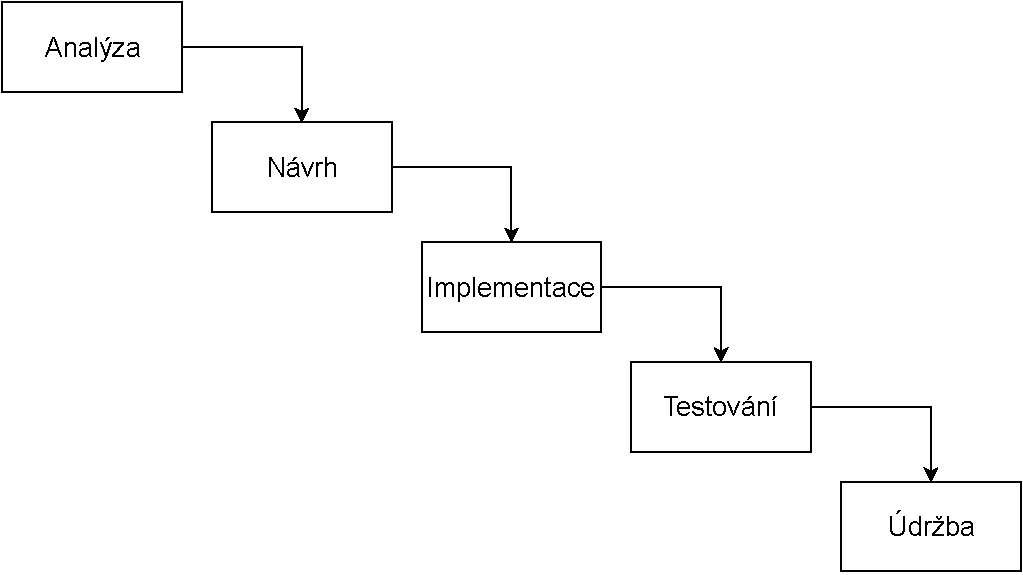
\includegraphics[width=0.8\textwidth]{obrazky-figures/waterfall-wide.pdf}
	\caption{Grafické znázornění posloupnosti jednotlivých procesů tradiční metodiky řízení projektů označované jako vodopádový model.}
	\label{img:waterfall}
\end{figure}

U tradičních metodik je předpokladem, že se k dokončeným fázím projektu již nebude nutné vracet. Takový předpoklad lze aplikovat na mnoho odvětví. Příkladem budiž stavba budovy, u které je nutné nejprve řádně celý projekt naplánovat a zdokumentovat. Jakmile samotná stavba započne, větší změny oproti původnímu projektu vznikají velmi zřídka. V oblasti informačních technologií, obzvláště při vývoji softwaru, však odchýlení od původního plánu nebývá žádnou výjimkou. Řízení projektů tohoto typu pomocí striktních tradičních metodik je tedy často obtížné a značně neefektivní~\cite{bib:agile-vs-traditional-what}.

V dnešní době se stává častěji než tomu bylo v minulosti, že se softwarové projekty během vývoje mění, narůstají jejich požadavky, přibývají funkce a to vše i během jejich vývoje. Tento trend se týká především webových systémů. Jako reakce na tyto náhlé změny byly v devadesátých letech stvořeny právě agilní metodiky~\cite{bib:agile-history}. 

\subsection{Agilní metodiky řízení projektů}
Agilní metodiky jsou skupina metod řízení projektů určena především pro vývoj softwaru. Jak název napovídá, jedná se o metodiky, které se vyznačují dynamičností a flexibilitou.

Veřejný zájem o tyto metodiky začal až v pozdních devadesátých letech~\cite{bib:agile-mobile}. V roce 2001 se v Utahu sešlo sedmnáct zastánců agilních metodik a sestavilo Manifest agilního vývoje software\footnote{ Manifest agilního vývoje: \url{https://agilemanifesto.org/iso/cs/manifesto.html}}, který vystihuje čtyři hlavní zásady těchto metod~\cite{bib:agile-manifest}.
\begin{itemize}
  \item Jednotlivci a interakce před procesy a nástroji
  \item Fungující software před vyčerpávající dokumentací
  \item Spolupráce se zákazníkem před vyjednáváním o smlouvě
  \item Reagování na změny před dodržováním plánu
\end{itemize}

Tyto metodiky jsou více zaměřené na lidi a na jejich vzájemnou komunikaci. To je jedním z důvodů, proč jsou agilní metodiky vhodné především pro menší týmy. Díky absenci sekvenčního řazení procesů vývoje tyto metody také zvyšují efektivitu nepředvídatelných a stále se měnících projektů. Vypuštěním striktního plánování je také možné projekt mnohdy dokončit rychleji než použitím tradičních metodik.

Vývoj řízený agilními metodikami probíhá iterativně a inkrementálně. Na začátku vývoje se určí základní požadavky a postupnými cykly se tyto požadavky zdokonalují. Jedna iterace takového vývoje trvá zpravidla jeden týden až měsíc. Během této iterace proběhne celý cyklus vývojových procesů (podobný vodopádovému modelu znázorněného diagramem~\ref{img:waterfall}). Dokončením iterace vzniká prototyp, který může být prezentován zákazníkovi. Díky tomu zákazník získává přesnější představu o podobě produktu a lze včas odhalit nedostatky požadavků, které dříve nebyly známy~\cite{bib:agile-impact}. 
Průběh tohoto iterativního vývoje je znázorněný diagramem~\ref{img:agile}.

\begin{figure}[H]
	\centering
	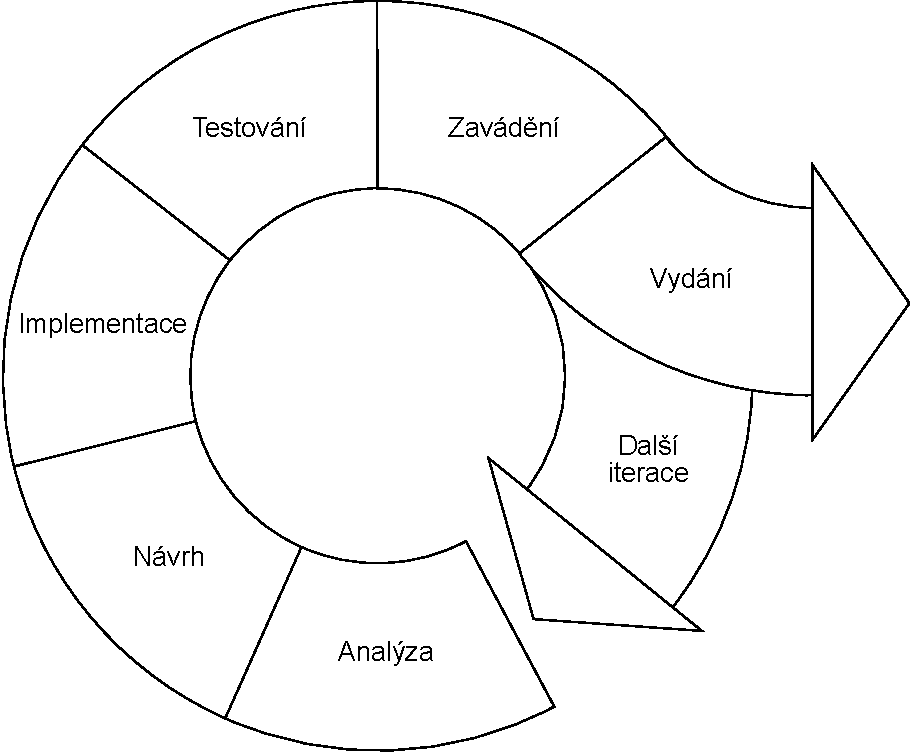
\includegraphics[width=0.7\textwidth]{obrazky-figures/agile.pdf}
	\caption{Grafické znázornění posloupnosti jednotlivých procesů agilních metodik řízení projektů. Cyklus začíná procesem analýza a pokračuje až po proces zavádění, kdy je projekt buďto hotov a následuje jeho vydaní nebo proběhne další iterace a celý cyklus se znovu opakuje.}
	\label{img:agile}
\end{figure}

Mezi populární agilní metodiky patří například Scrum, Lean Developmet, Extrémní programování (angl. \emph{Extreme Programming} nebo také XP), Crystal, Vlastnostmi řízený vývoj (angl. \emph{Feature Driven Development} neboli FDD) a v neposlední řadě také Kanban.

Jedna ze studií na toto téma vydána roku 2015 uvádí, že ze 1386 sledovaných projektů 65\% z nich využilo během vývoje agilní metody a 6\% projektů bylo dokončeno téměř pouze s použití agilních metod. Závěrem této studie je také pozorování poukazující na fakt, že čím větší poměr agilních metodik byl při vývoji použit, tím úspěšnější dané projekty byly~\cite{bib:agile-work}.

\subsection{Metodika Kanban}
Kanban je slovo převzaté z japonského jazyka, kde znamená \uv{cedule}. Toto slovo je taktéž spjato s poslední výzvou k objednávce před uzavřením podniku (sundáním cedule). Takovou objednávku lze označit jako \uv{na poslední chvíli} nebo také jako objednávku \uv{tak akorát na čas}~\cite{bib:dict-kanban}. 

Tak akorát na čas (anglicky \emph{Just-in-time}) je filozofie řízení výroby, vyvinuta v sedmdesátých létech japonskou automobilovou společností Toyota Motor Corporation\footnote{Toyota Motor Corporation: \url{https://global.toyota/en/}}. Hlavní myšlenkou toho přístupu je mít přesné množství materiálu, na správném místě a ve správný čas. Díky tomu dochází k redukci množství materiálu, který aktuálně není zpracováván a nemělo by docházet k jeho přebytečnému hromadění~\cite{bib:just-in-time}. Jedním z nástrojů této filozofie je právě metodika Kanban, její tehdejší provedení je možné vidět na fotografii~\ref{img:kanban-toyota}.

\begin{figure}[H]
	\centering
	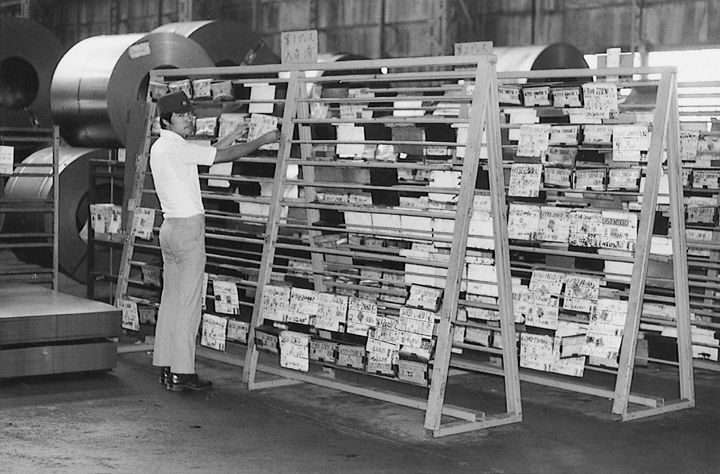
\includegraphics[width=\textwidth]{obrazky-figures/toyota-kanban.jpg}
	\caption{Původní provedení kanbanu v továrně společnosti Toyota Motor Corporation \emph{Převzato z~\cite{bib:toyota-history}}.}
	\label{img:kanban-toyota}
\end{figure}

Metodika Kanban je nástroj pro vizuální kontrolu práce a jejího toku jednotlivými fázemi procesu. Kanban může být realizován jak fyzicky (například tabule s nalepovacími papírky viz fotografie~\ref{img:kanban-whiteboard}), tak i digitálně (například pomocí aplikací uvedených v kapitole~\ref{sec:apps}). 

Ať je nástěnka Kanban digitální či nikoliv, ve většina případů se skládá ze stejných částí, jen v jiném provedení. Nejčastěji se lze setkat s typem, kdy na se na horizontální ose nachází pojmenované sloupce představující jednotlivé fáze procesu. Do těchto sloupců jsou umístěny nejrůznější karty, reprezentující jednotlivé úkoly. Rozmístění karet mezi sloupci se odvíjí od aktuálního stavu úkolu.

Nejjednodušší variantou takových sloupců může být například trojce sloupců nazvaných \uv{zásobník}, \uv{v procesu} a \uv{hotovo}. První ze sloupců nazvaný \uv{zásobník} je místo, kde se hromadí úkoly, na kterých se ještě nezačalo pracovat. Jakmile práce na daném úkolu započne, jeho karta je přesunuta do dalšího sloupce s označením \uv{v procesu}. Obdobně je tomu při dokončení úkolu, kdy je jeho karta opět přemístěna do jiného sloupce, tentokrát do sloupce \uv{hotovo}. Názorná ukázka této nástěnky je vidět na fotografii~\ref{img:kanban-whiteboard}.

\begin{figure}[H]
	\centering
	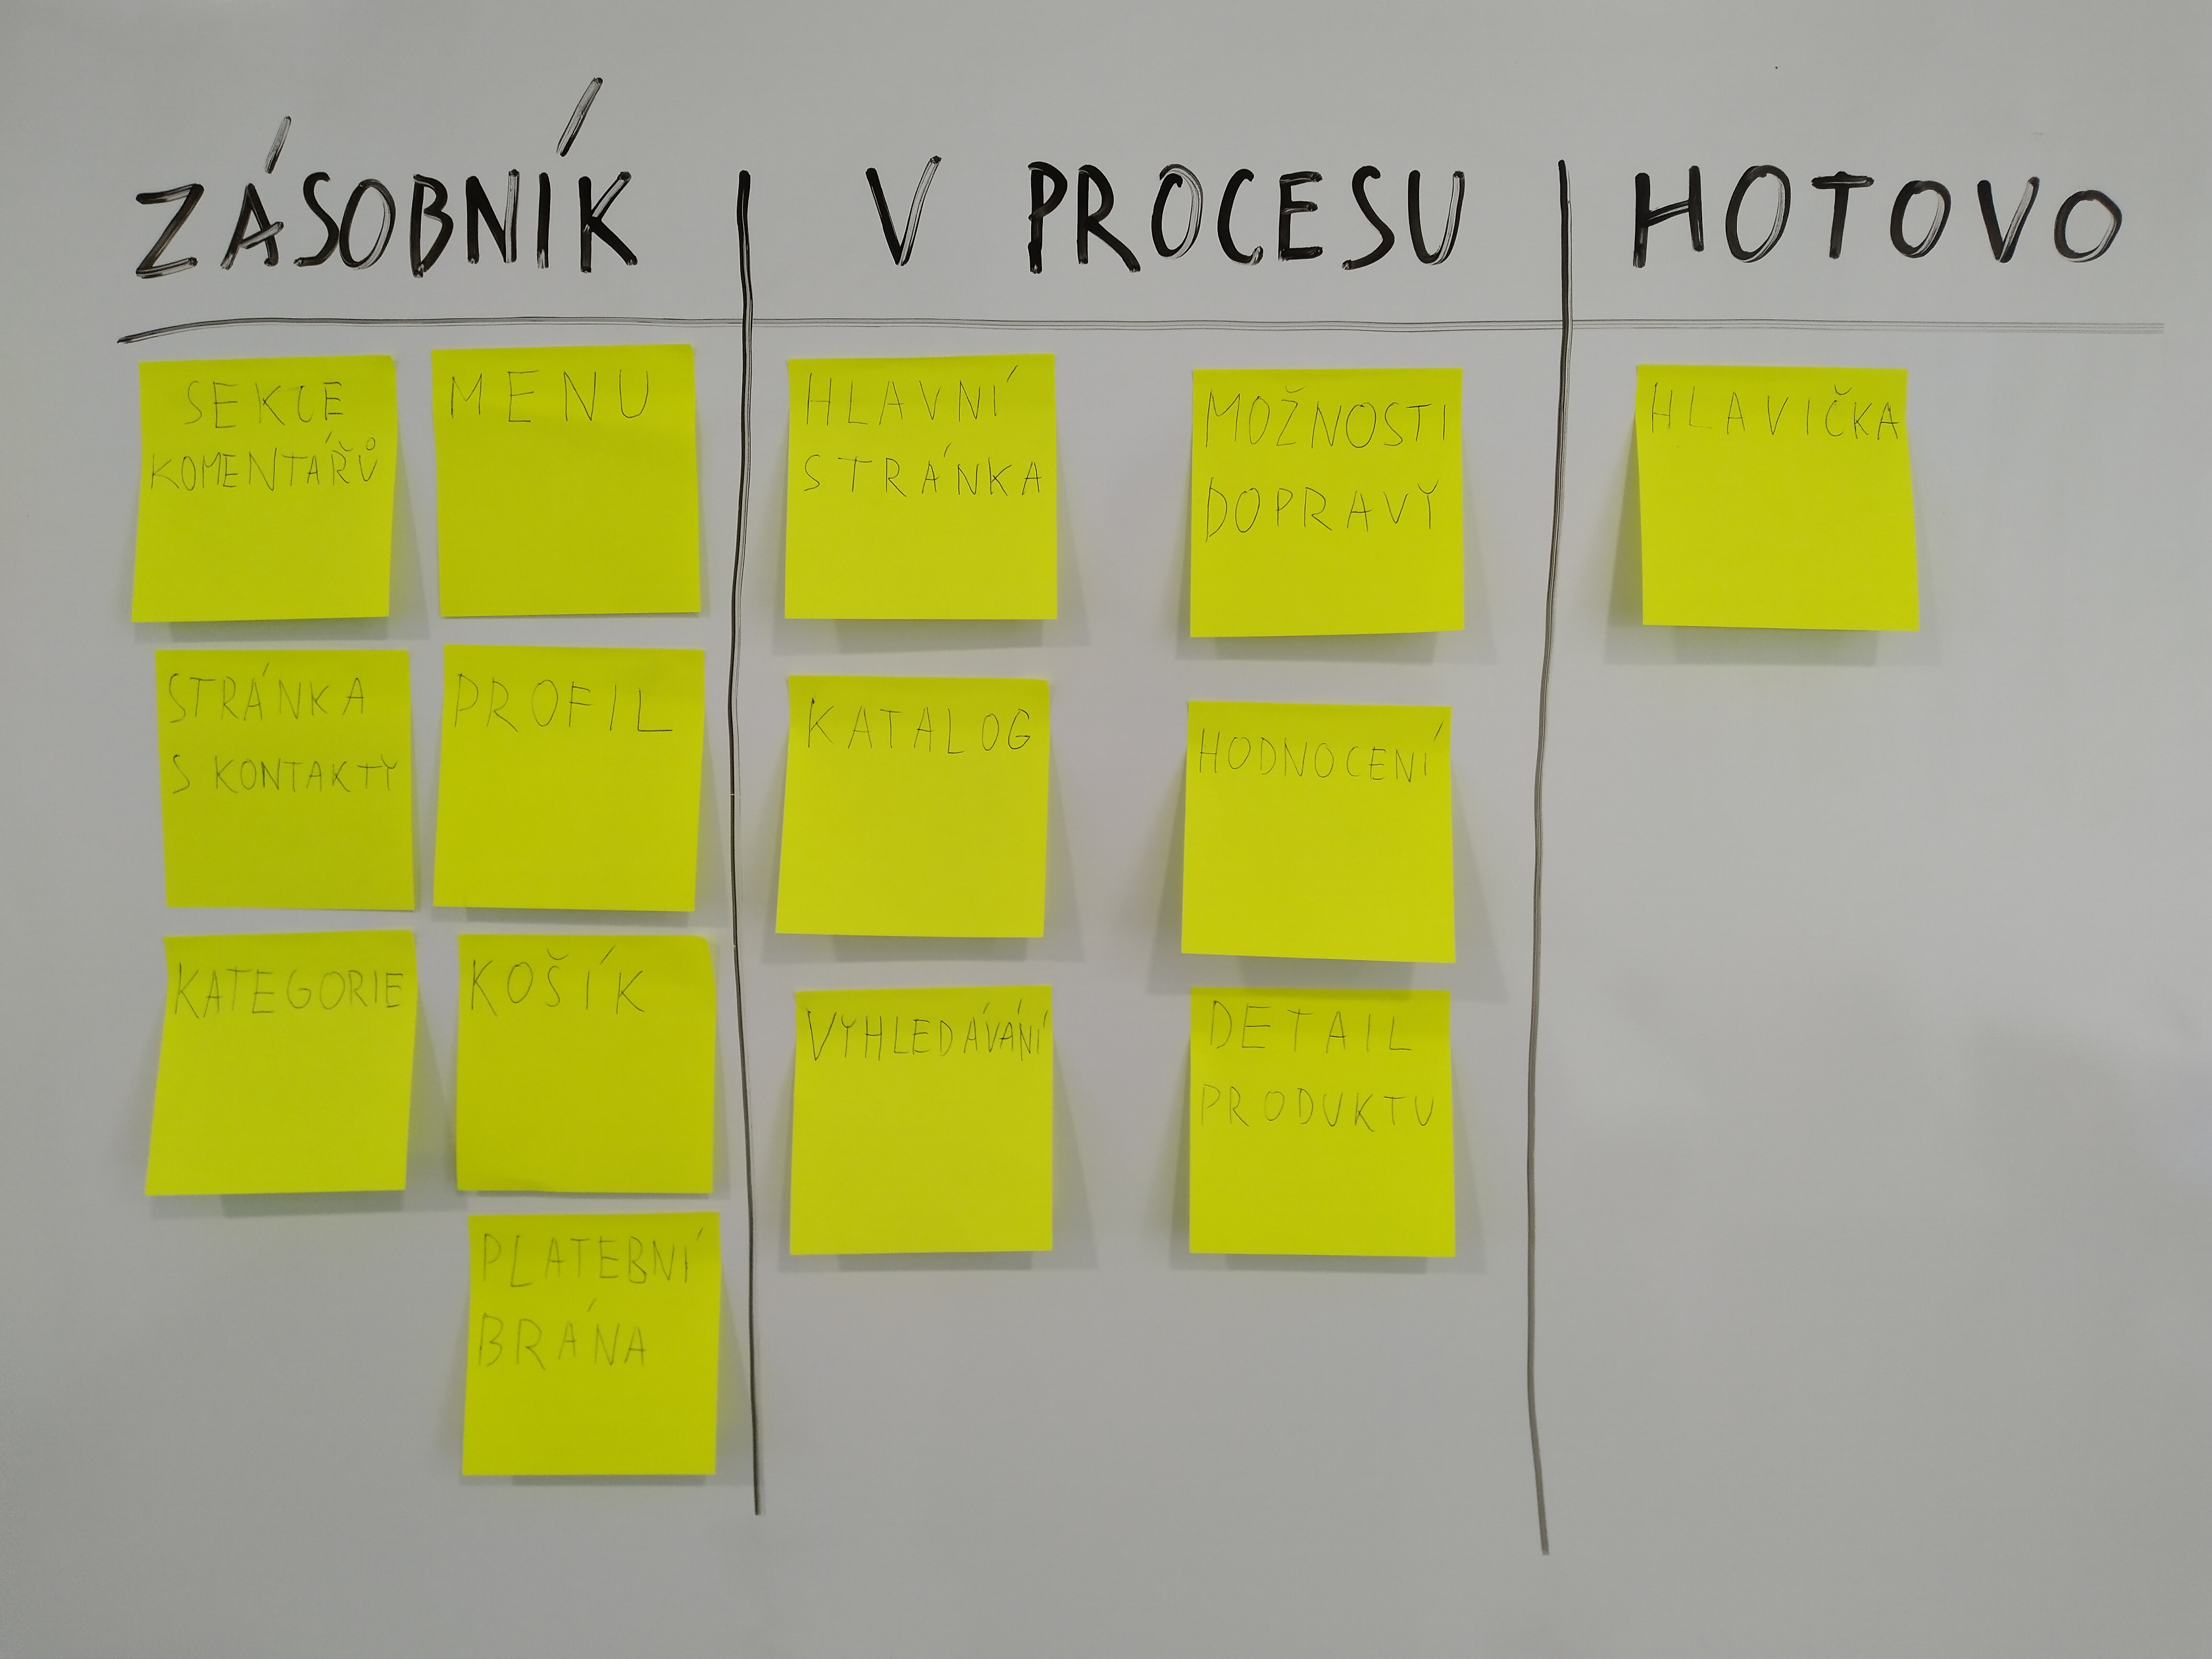
\includegraphics[width=\textwidth]{obrazky-figures/kanban-sticky-note}
	\caption{Nástěnka typu Kanban realizována pomocí nalepovacích papírků na magnetické tabuli.}
	\label{img:kanban-whiteboard}
\end{figure}

V praxi je takřka nemožné setkat se s takto jednoduchým provedením. Proces výroby či vývoje je třeba rozdělit na jednotlivé části. Při vývoji softwaru bývají často využívány sloupce \uv{návrh}, \uv{vývoj}, \uv{testování} a další.  

Pokud jednu nástěnku využívá více oddělení společnosti, lze se mnohdy setkat i s dalším rozlišením úkolů. Jedná se o takzvané plavecké dráhy (angl. \emph{swimlanes}). Úkoly jsou pak rozděleny nejen do sloupců (značících procesy), ale i do vodorovných řádků, které nejčastěji představují jednotlivá oddělení společnosti či týmy. 

V dnešní době, jak u mnoha věcí, převažuje digitální provedení Kanban nástěnek. Její výhodou je především větší přehlednost, vzdálená přístupnost, jednoduší manipulace a hlavně možnost připojovat k jednotlivým kartám podrobnější popis, komentáře, obrázky a další dokumenty. Nicméně i fyzická varianta má své výhody. Jedna z nich je fakt, že je stále na očích a nelze ji skrýt jako například záložku v prohlížeči. Toto provedení může taktéž podněcovat k vetší komunikaci mezi týmy a to jsou důvody proč tuto variantu využívají například ve společnosti Optimizely\footnote{Optimizely: \url{https://www.optimizely.com/about/}}~\cite{bib:kanban-atlassian}.

Díky využití metodiky Kanban a jejího přehlednému vyobrazení úkolů získávají jednotliví členové týmu lepší přehled o prací svých kolegů. Tento fakt může také vést k lepší prioritizaci úkolů a především odpadá čas ztracený komunikací v momentě kdy nastane změna úkolu čí jeho priority~\cite{bib:kanban-101}.
Kanban svou podstatou také dokáže poukázat na problematické procesy, které zpomalují celkový chod výroby či vývoje~\cite{bib:kanban-and-scrum}.

Často se u metodiky Kanban lze potkat s limitováním probíhající práce (anglicky \emph{Work in Progress]} či zkráceně WIP). Jedná se o omezení, kdy dán maximální počet úkolů pro určitou fázi procesu (sloupec nástěnky). Například lze stanovit limit souběžného pracování maximálně na třech grafických návrzích. Toto omezení má pozitivní dopad především na snížení nutnosti věnovat se více projektům naráz, díky čemuž se lze na jednotlivé úkoly lépe soustředit a tím může být docíleno rychlejšího a kvalitnějšího výsledku~\cite{bib:kanban-101}.

\section{Aplikace s podobným zaměřením}\label{sec:apps}
Jelikož metodika Kanban existuje již několik několik desítek let, lze v dnešní době nalézt celou řadu programů a webových aplikací, které je možné pro aplikování této metodiky využít. V této podkapitole je několik takových aplikací stručně přiblíženo a jsou vyzdviženy některé jejich klíčové vlastnosti. Pro bližší představu o podobě těchto aplikací je každá doprovázena jejím snímkem. Mezi uvedenými aplikacemi lze nalézt dva populární zástupce z řad produktů společnosti Atlassian -- aplikace Trello a Jira. Třetí představenou aplikací je o něco méně známá aplikace Kanboard, která je však v současné době využívaná společností SEACOMP s.r.o. V závěru kapitoly je obsaženo stručné shrnutí rozdílů těchto tří aplikací a možné důvody vedoucí ke zvolení právě jedné z uvedených aplikací.

\subsection{Trello}
Trello\footnote{Trello: \url{https://trello.com}} je především webová aplikace provozovaná v současné době společností Atlassian\footnote{Atlassian: \url{https://www.atlassian.com}}. Historie této aplikace sahá až do roku 2011, kdy byla veřejně spuštěna jako webová aplikace a také jako aplikace pro platformu iOS. K dnešnímu dni je aplikaci Trello možné navíc využít i na mobilní platformě Android nebo jako desktopová aplikace pro operační systémy Microsoft Windows či macOS. 

Během několika let své existence se aplikace stala velice populární a použilo ji několik milionů uživatelů. K věhlasným společnostem, které tuto aplikaci využívají patří například technologický gigant Google\footnote{Google: \url{https://about.google/}}, softwarová společnost Red Hat\footnote{RedHat: \url{https://www.redhat.com/en/about/company}} nebo platforma pro skupinové financování Kickstarter\footnote{Atlassian: \url{https://www.kickstarter.com/about}}~\cite{bib:trello-about}. 

Svou velkou popularitu si aplikace zasloužila především přívětivým uživatelským rozhraním a jednoduchostí použití. Od první návštěvy stránky k práci na své první Kanban nástěnce uživatele dělí doslova minuty. Pro základní použití navíc bez problému vystačí bezplatná verze aplikace. Díky těmto faktům aplikace není využívána pouze softwarovými společnostmi, ale lze ji použít například i jako osobní seznam úkolů~\cite{bib:jira-vs-trello}.

Trello nabízí řadu vylepšení, díky kterým je možné nástěnku rozšířit o funkce z aplikací třetích stran. 
V bezplatné verzi lze však využít pouze jedno takové vylepšení~\cite{bib:trello-pricing}.
Nástěnka je umístěna na serverech poskytovatele a službu nelze provozovat na svém vlastním serveru. Nicméně mobilní aplikace umožňují pracovat s nástěnkami i bez přístupu k internetu~\cite{bib:trello-common}.

\begin{figure}[H]
	\centering
	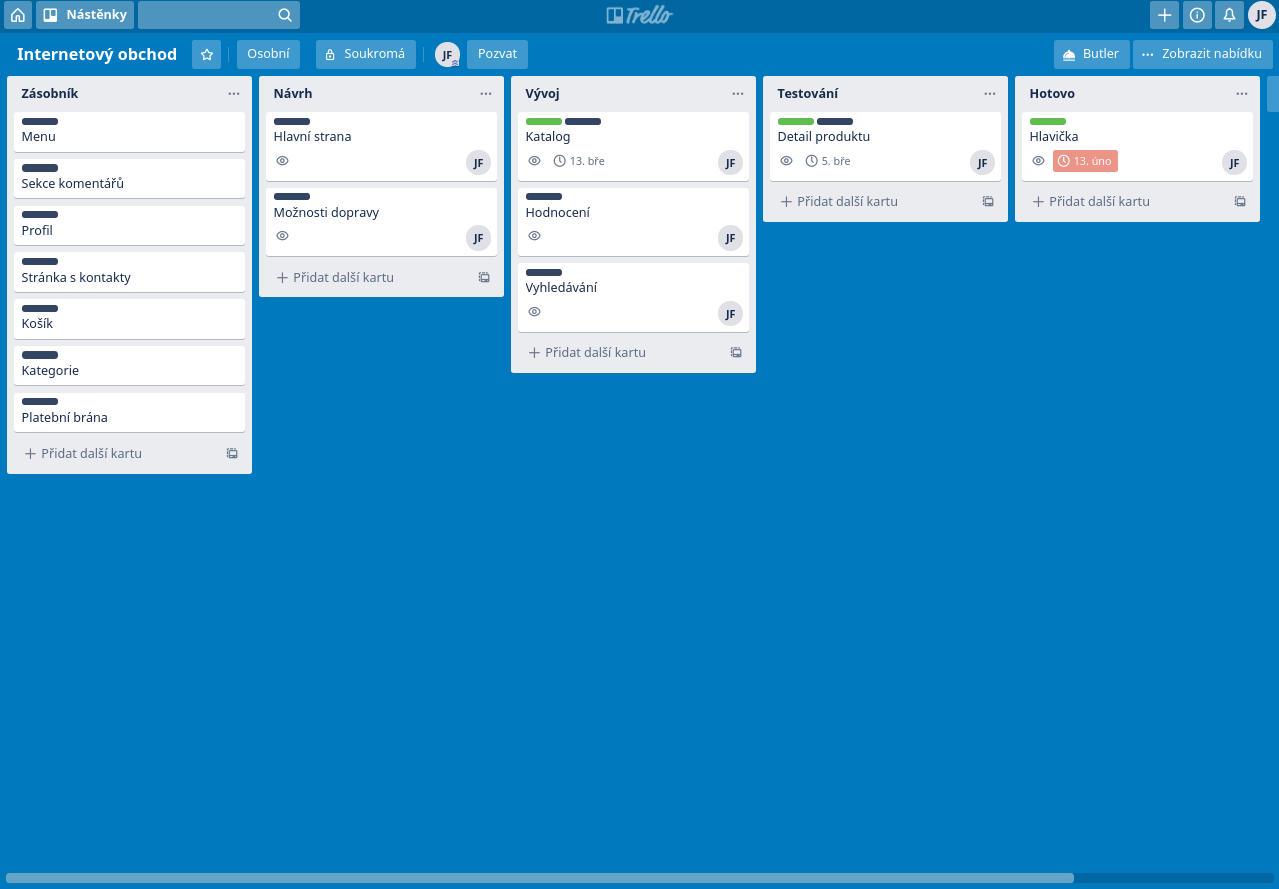
\includegraphics[width=\textwidth]{obrazky-figures/trello.png}
	\caption{Vzorová Kanban nástěnka ve webové aplikaci Trello zaměřená na vývoj internetového obchodu.}
\end{figure}

\subsection{Jira}
Jira\footnote{Jira: \url{https://www.atlassian.com/cs/software/jira}} je řada produktů společnosti Atlassian, určená ke správě práce v nejrůznějších typech týmů. Nástěnka Kanban je součást například produktu Jira Software, který je, jak název vypovídá, zaměřen především na vývojáře softwaru. 
% https://www.atlassian.com/software/jira/guides/getting-started/overview#jira-software-hosting-options

S nástěnkou lze pracovat jak v prohlížeči, tak i pomocí vlastního programu, který je k dispozici pro operační systémy Microsoft Windows, Linux i macOS. K dispozici jsou také mobilní aplikace pro operační systém iOS i Android. 

Jednou z funkcí, kterou Jira disponuje, je možnost vygenerování řady grafů a přehledů. V základní verzi bez přídavných modulů lze také tvořit dílčí úkoly a vzájemné závislosti jednotlivých úkolů. Základní funkcionalitu aplikace lze rozšířit využitím placených i bezplatných doplňku, které jsou k dispozici na oficiálním tržišti.

Díky tomu, že je aplikace určená pro softwarové vývojáře je v této aplikaci mimo klasické nástěnky možné také přepnout režim zobrazení na variantu určenou pro agilní metodiku zvanou Scrum, která cílí na dokončení úkolů v rámci iterace cyklu vývoje~\cite{bib:trello-vs-jira-2020}.

Nástěnka může být na rozdíl od aplikace Trello umístěna jak na serverech poskytovatele, tak i na vlastním serveru.

Tato aplikace je využívána více něž 65 tisíci zákazníky po celém světě mezi které se řadí například internetovou aukční síň eBay\footnote{eBay: \url{https://www.ebayinc.com/company/}}, služba pro streamování hudby Spotify\footnote{Spotify: \url{https://newsroom.spotify.com/company-info/}}, společnost vyrabějící síťové prvky Cisco\footnote{Cisco: \url{https://www.cisco.com/c/en_uk/index.html}} nebo aplikace pro pronájem ubytování Airbnb\footnote{Airbnb: \url{https://news.airbnb.com/about-us/}}~\cite{bib:jira-homepage}.

\begin{figure}[H]
	\centering
	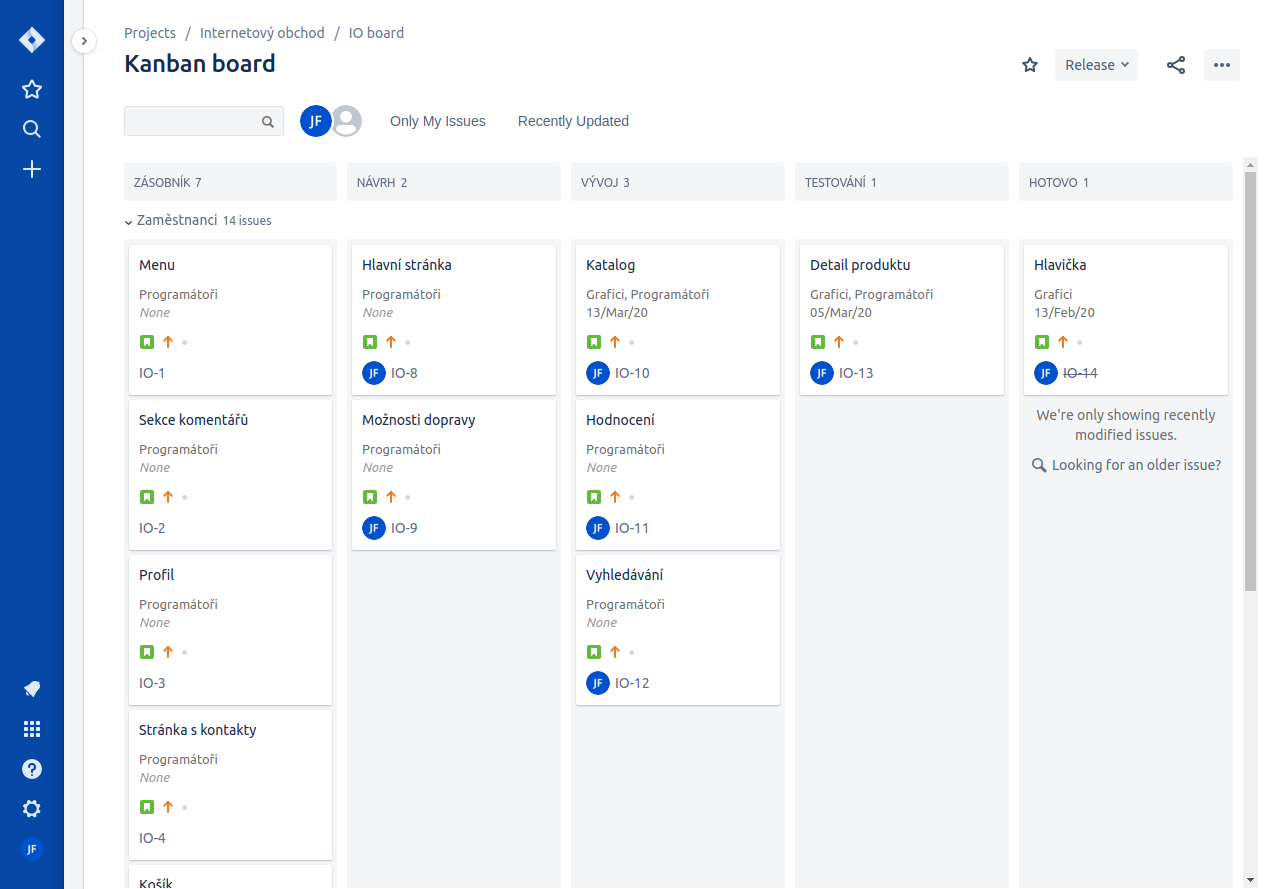
\includegraphics[width=\textwidth]{obrazky-figures/jira.png}
	\caption{Vzorová Kanban nástěnka ve webové aplikaci Jira Software zaměřená na vývoj internetového obchodu.}
\end{figure}

\subsection{Kanboard}
Kanboard\footnote{Kanboard: \url{https://kanboard.org}} je bezplatná webová aplikace s otevřeným zdrojovým kódem. Jejím tvůrcem je Frédéric Guillot, nicméně zdrojové kódy jsou volně k dispozici na portálu GitHub\footnote{Repozitář Kanboard na platformě GitHub: \url{https://github.com/kanboard/kanboard}}, kde se k vývoji připojilo dalších 270 lidí~\cite{bib:kanboard-github}. Aplikace je napsaná především v jazyce PHP a JavaScript. K provozování této aplikace je nutné použít vlastní webový server. Kanboard uživatelům nenabízí žádné přepychové uživatelské rozhraní, ale naopak se zaměřuje na jednoduchost a minimalismus~\cite{bib:kanboard}.

Mimo základní funkce metodiky Kanban tato aplikace umožňuje také vyhledávat úkoly za pomocí vlastního dotazovacího jazyka. Částečně také umožňuje práci s nástěnkou automatizovat pomocí konfigurovatelných akcí.

Vzhledem k otevřenému zdrojovému kódu lze aplikaci v případě potřeby upravit na míru vlastním potřebám. Součástí aplikace je však i rozhraní pro zásuvné moduly. Několik takových modulů lze nalézt i přímo na oficiální stránce\footnote{Zásuvné moduly pro Kanboard: \url{https://kanboard.org/plugins.html}}, avšak nepodléhají žádnému schvalovacímu procesu a není zaručena jejich kompatibilita.

Aplikace však nenabízí žádný program či mobilní aplikaci. Jediný přístup k nástěnce je tedy pomocí internetového prohlížeče.

\begin{figure}[H]
	\centering
	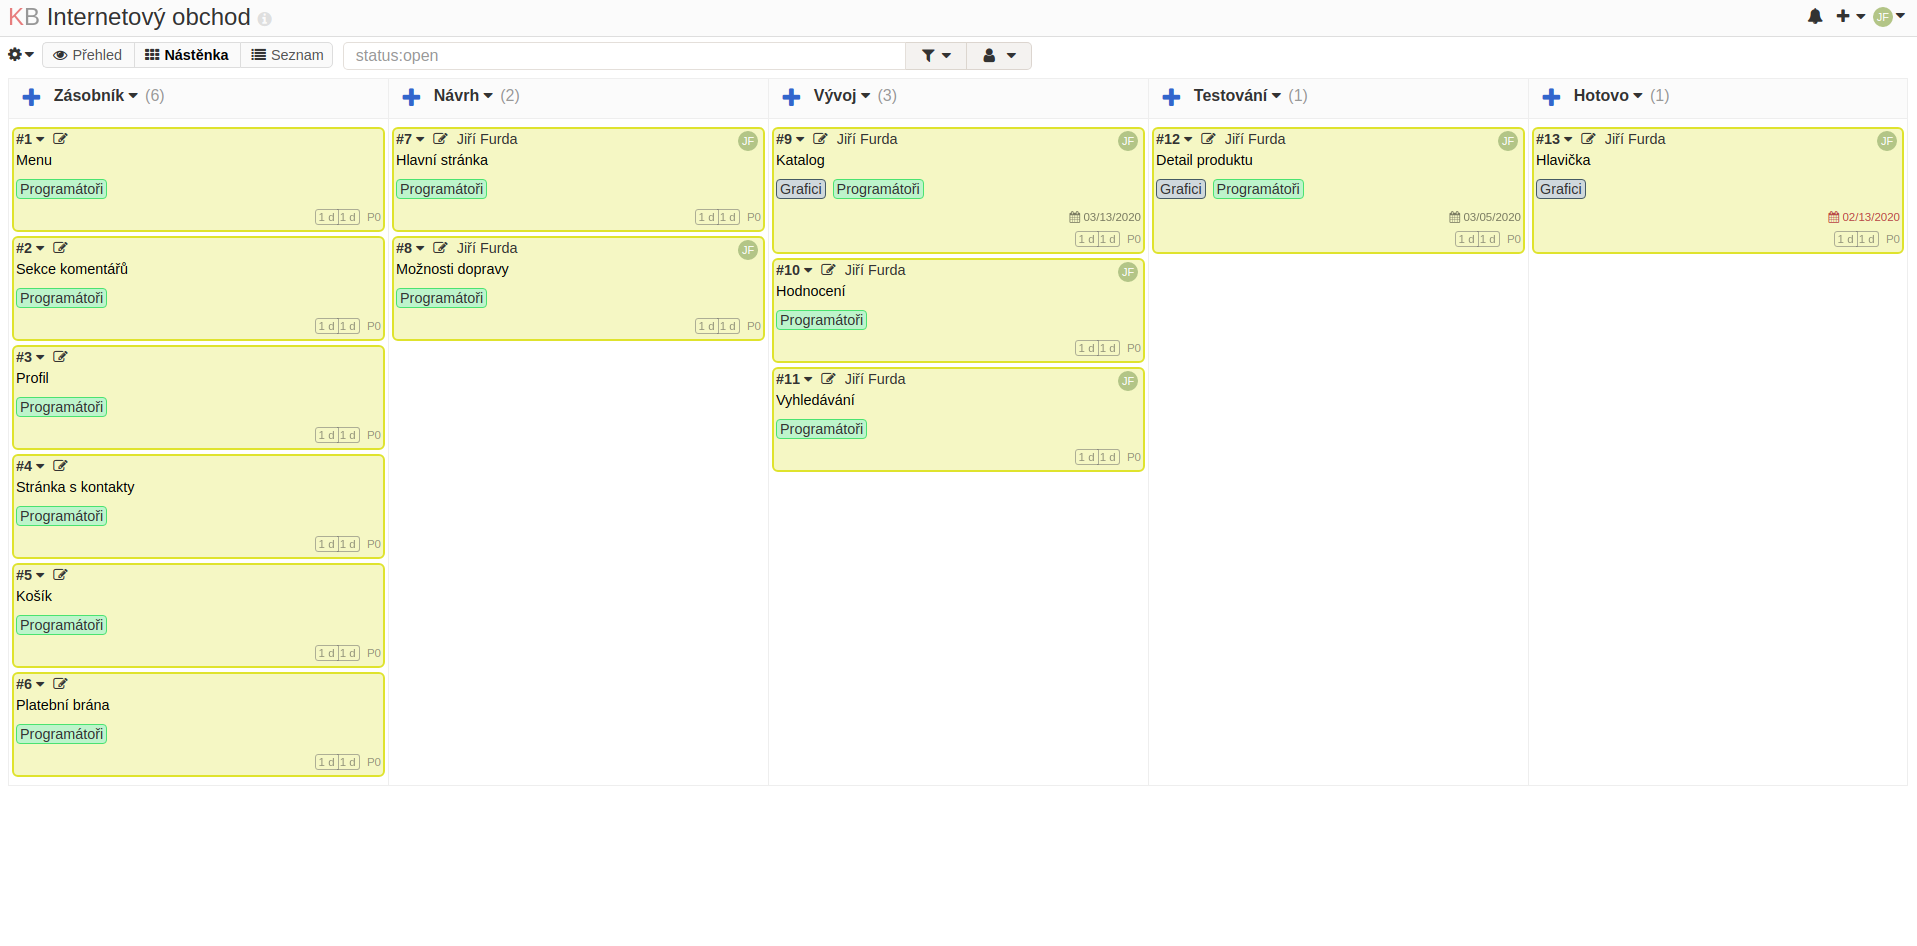
\includegraphics[width=\textwidth]{obrazky-figures/kanboard.png}
	\caption{Vzorová Kanban nástěnka ve webové aplikaci Kanboard zaměřená na vývoj internetového obchodu.}
\end{figure}

\subsection{Souhrn rozdílů}

Základní principy nástěnky Kanban jsou součástí všech tří uvedených aplikací. Malou odchylkou je aplikace Trello, která neumožňuje úkoly rozřadit do plaveckých drah. Této funkcionality lze docílit pouze instalací zásuvného modulu do prohlížeče, což zcela jistě není nejvhodnější řešení.

Představené aplikace se mezi sebou liší například cenou, možnostmi provozování, dostupností zdrojového kódu, existencí mobilní aplikace, dostupností technickou podporou či přívětivostí uživatelského prostředí. Srovnání několik těchto vlastností je přehledně uvedeno v tabulce~\ref{tab:kanban-sum}. 

\begin{table}[H]
\centering
\caption{Srovnání rozdílů mezi několika aplikacemi typu Kanban}
\label{tab:kanban-sum}
\begin{tabular}{ |l|c|c|c|c| } 
\hline
Aplikace & Cena\footnotemark & Vzdálené úložiště & Vlastní úložiště & Otevřený zdrojový kód  \\
\hline
Trello & 0--20,83 dolarů~\cite{bib:trello-pricing} & Ano & Ne & Ne \\ 
Jira & 0--14 dolarů~\cite{bib:jira-pricing} & Ano & Ano & Ne \\ 
Kanboard & Zdarma & Ne & Ano & Ano \\ 
\hline
\end{tabular}
\end{table}
\footnotetext{Cena na uživatele za měsíc}

Z důvodu ochrany firemního tajemství mohou být preferovány služby Jira a Kanboard, jelikož je možné je provozovat přímo na svém vlastním serveru. Konkrétně u aplikace Kaboard může tato vlastnost však představovat pro řadu uživatelů nevýhodu. Aplikaci totiž není možné jednoduše provozovat na serverech poskytovatele. Uživatel musí mít k dispozici server, kde bude aplikace provozována a to se může stát bariérou pro méně pokročilé uživatele počítače.

Kanboard však jako jediná z tří uvedených aplikací disponuje otevřeným zdrojovým kódem. Umožňuje tak větší zásahy do aplikace než je tomu v případě dalších dvou aplikací, kde lze úpravy řešit pouze pomocí doplňků.

Co se ceny týče, všechny aplikace lze provozovat v jistém měřítku zdarma. Trello v bezplatné verzi omezuje počet týmových nástěnek a Jira zase využívá limit uživatelů. Oproti tomu Kanboard, je zcela zdarma. Jediné reálné náklady tedy může představovat provoz serveru. Při provozování aplikace Jira tímto způsobem je třeba uhradit jednorázový poplatek, jehož cena se odvíjí od počtu uživatelů. Použití aplikace Kanboard se tedy může jevit jako nejlepší volba, každopádně v tomto případě je ztracena dostupnost technické podpory. V korporačním prostředí to může být důležitý požadavek, protože výpadek klíčového nástroje pro řízení projektů představuje obrovské riziko pro bezproblémový chod společnosti.

Slabší stránkou aplikace Kanboard je na první pohled uživatelské rozhraní. Nejedná se však pouze o vzhled aplikace. Rozhraní obsahuje i mnoho prvků, které nejsou řešeny pomocí asynchronních požadavků, a to může být uživateli vnímáno jako nepohodlné či zastaralé.

Každá z uvedených aplikací tedy obsahuje řadu výhod i nevýhod, nelze tedy jednoznačně určit tu nejlepší. Výběr závisí na konkrétních požadavcích společnosti či týmu, který ji bude využívat. Nicméně za zmínku stojí fakt, že 83\% společností ze žebříčku Fortune 500\footnote{Fortune 500: \url{https://fortune.com/fortune500/}}, který sdružuje 500 společností ze Spojených států Amerických s nejvyšším hrubým obratem, využívá produkty právě společnosti Atlassian~\cite{bib:atlassian-customers}.



\section{Společnost SEACOMP s.r.o.}
SEACOMP s.r.o. je česká společnost věnující se již více než dvacet let tvorbou softwarových produktů. Společnost se zabývá především informačními systémy v oblasti logistiky, zdravotnictví, správy budov a řízení projektů~\cite{bib:seacomp-portfolio}.


\subsection{Současný produkt}
Jedním z mnoha produktů společnosti SEACOMP s.r.o. je systém SSB (SEACOMP SYSTEM BUILDER), určený pro snadnou tvorbu komplexních informačních systémů. Jedná se o počítačový program napsaný za použití technologie .NET.

V loňském roce se v rámci své diplomové práce Bc. Adam Teršl věnoval implementaci webového klienta pro tento systém. Výsledkem jeho snažení byla webová aplikace SSB4Web využívající především rámec Angular. Aplikace je schopna komunikovat se serverem systému SSB a díky zásuvným modulů umožňuje prezentaci základních typů dat, které tvoří základ tohoto systému~\cite{bib:tersl}. Desktopová verze klienta však obsahuje celou řadu dalších specializovaných zásuvných modulů, které pro webovou verzi klienta dosud nebyly implementovány. Jedním z těchto modulů je právě nástroj KANBAN board pro optimalizaci spolupráce týmů, jehož implementace je cílem mé práce. 

Původní nástroj však svou funkcionalitou pro pokročilejší řízení projektů již nestačí. Z tohoto důvodu se v rámci interního projektového řízení začal ve společnosti SEACOMP s.r.o. používat nástroj Kanboard, který byl upraven a obohacen o některé specializované funkce. Tento nástroj však pracuje mimo ekosystém SSB. Přáním společnosti je mít k dispozici nástroj, který umožňuje pokročilejší práci s nástěnkou typu Kanban a tento nástroj mít plně integrován do produktu SSB4Web. Z tohoto důvodu bylo vypsané toto téma bakalářské práce.


\subsection{Požadavky na aplikaci}
Z důvodu ochrany obchodního tajemství však není možné zveřejnit zdrojové kódy programu SSB. Pro řešení této bakalářské práce je tudíž nejprve nutné vytvořit zjednodušenou verzi toho systému. Ta nese označení SSBLite a dle požadavku zadavatele je psána v jazyce C\#, konkrétně za použití ASP.Net Core. Tato část slouží jako server a komunikuje s klienty skrze aplikační rozhraní REST.

Podoba aplikačního rozhraní z důvodu budoucí integrace do systému SSB4Web musí odpovídat podobě používané právě v této zmíněné webové aplikaci. Samotná integrace však na přání společnosti není předmětem této práce, aplikaci je proto i přes budoucí integraci nutno vytvořit jako samostatnou webovou aplikaci obsahující například i autentizaci uživatelů a další komponenty.

Dále je požadováno, aby webová aplikace používala stejné technologie jako původní SSB4Web, tedy rámec Angular s knihovnou pro správu stavu NgRx. Výjimkou je v tomto případě knihovna použitá pro uživatelské rozhraní, kdy původní diplomová práce využívala knihovnu PrimeNG\footnote{PrimeNG: \url{https://primefaces.org/primeng/}}. Po dokončení této práce však bylo společností požadováno knihovnu nahradit za balík komponent DevExtreme. Tento balík je tedy při implementaci práce rovněž využít.

Od samotné funkcionality aplikace je přirozeně očekáváno standardní chování aplikací toho typu jako je vytváření, mazání, editace a přesuny karet. Nástěnka kromě sloupců musí umět pracovat také s plaveckými drahami a obě tyto struktury musí být v aplikaci konfigurovatelné. Ke kartám je nutné mít možnost přiřadit štítky, které taktéž musejí být konfigurovatelné. Veškeré akce týkající se karet musí byt zapisovaný a je třeba umožnit zobrazení historie jednotlivých karet.
Serverová část aplikace musí načítat konfiguraci vydefinovanou mimo zdrojový kód aplikace. Pro autentizaci uživatele je požadováno využívat standard JWT.




\chapter{Technologie}
V této kapitole jsou ve stručnosti přiblíženy technologie a techniky využité při tvorbě této práce. 
V dnešní době popularita webových aplikací stále roste a to na úkor klasických desktopových aplikací~\cite{bib:web-apps-popular}. Tohoto trendu si je vědoma i společnost SEACOMP s.r.o., a proto je jejím záměrem vytvořit webovou aplikaci typu Kanban. Všechny použité technologie jsou tedy právě webového charakteru.

Úvod podkapitoly je věnován klientské části aplikace. Je zde popsán princip jednostránkových aplikací, programovací jazyk JavaScript, jeho typová nástavba TypeScript, rámec Angular a jeho knihovny NgRx a DevExtreme.

Dále jsou zmíněny technologie zajišťující propojení klientské části aplikace s části serverovou. Toho je docíleno díky aplikačnímu rozhraní REST a standardu JWT, která zajišťuje autentizaci uživatelů a autorizaci jejich požadavků.

V poslední části podkapitoly je zase popsána serverová část. Ta se skládá z technologie ASP.NET, která zpracovává požadavky zaslané z klientské části aplikace a překládá je na dotazy databáze, která využívá technologii PostgreSQL.


\section{Jednostránkové aplikace}\label{sec:spa}

\emph{Tato kapitola čerpá z~\cite{bib:spa}}.

V raných dobách internetu se webové stránky skládaly ze statického obsahu. S popularizací elektronického obchodování se však objevila potřeba na stránkách zobrazovat i obsah dynamický. 

Této funkcionality lze docílit například díky technologii AJAX (Asynchronous JavaScript and XML). Technologie AJAX umožňuje komunikovat se serverem i po načtení stránky a tato komunikace probíhá na pozadí. Díky tomu není nutné při každé akci znovu načíst celou stránku, čímž je značně zredukován objem přenášených dat.

Při navštívení jednostránkové webové aplikace je ze serveru nejprve načtena počáteční zmenšená část stránky. Další obsah je vyžádán a načten zpravidla až na základě uživatelské interakce. Ve srovnání s vícestránkovými aplikacemi tak tento přístup umožňuje rychleji reagovat na požadavky uživatele.

Často se lze také setkat se změnou adresní řádky prohlížeče při pomyslném přechodu na jinou podstránku. Ve skutečnosti se však uživatel stále nachází na jedné stránce, jen byl její obsah aktualizován. Právě proto se zmíněný princip webových aplikací označuje jako jednostránkový.

Takovéto aplikace se zpravidla skládají z komponent. Pro tvorbu těchto aplikací se využívá jazyk JavaScript, nicméně vzhledem k jejich komplexnosti se v drtivé většině pro implementaci používá některých z rámců tohoto jazyka.

\section{JavaScript}
\blindtext

\subsection{TypeScript}
Samotný jazyk JavaScript však pro vývojáře může představovat překážku při implementaci rozsáhlých aplikací. Jedním z hlavních problémů je nepřehlednost kódu s dynamickým typováním proměnných.

Řešením tohoto problému je například nástavba TypeScript\footnote{TypeScript: \url{https://www.typescriptlang.org}}, která tento jazyk obohacuje o prvky běžně používané v jiných programovacích jazycích. Jedná se ku příkladu o moduly, třídy, rozhraní a v neposlední řadě statické typování. Díky tomu je možné vyvíjet robustnější aplikace~\cite{bib:typescript}.
 
Jelikož internetové prohlížeče jazyk TypeScript neznají, je využíván překladač, který kód překládá do jazyka JavaScript.

\subsection{Rámce jazyka JavaScript}
S použitím čistého jazyka JavaScript bez použití knihoven či rámců se dnes setkáváme zřídka. Zejména u větších projektů je psaní kódu v čistém jazyce JavaScript ve srovnáním s použítí knihoven a rámců velmi časově náročné~\cite{bib:vanilla-js}.

Nejslavnějším rozšířením toho jazyka je bezesporu knihovna jQuery\footnote{jQuery: https://jquery.com}. Ta usnadňuje zejména průchod a manipulaci objektového modulu dokumentu (angl. \emph{Document Object Model} neboli \emph{DOM}), zpracování událostí, animace a práci s asynchronními požadavky~\cite{bib:jquery}.

Knihovna jQuery však není určená pro tvorbu stále populárnějších jednostránkových aplikaci. Na ty se zaměřují zcela jiné rámce, kterých se v poslední době objevuje stále více.

V současné době se mezi tři nejpoužívanější rámce řadí Angular, React a Vue.js~\cite{bib:js-framework}. Za dvěma prvními těmito rámci stojí velké společnosti. Rámec Angular je dílem společnosti Google a rámec React zase společnosti Facebook. Autorem rámce Vue.js je však Evan You a komunita vývojářů po celém světě.

Nejmladším z těchto rámců je Vue.js i přes to se však těší větší oblibě než nejstarší uvedený rámec Angular. Angular jako jediný z uvedených rámců využívá nástavbu TypeScript. V ostatním rámcích ji sice také lze využít, není to však vyžadováno. Architektura všech tří rámců si je principem velmi podobná. Liší se opět pouze rámec Angular, který komponenty umožňuje rozdělit do jednotlivých modulů. Co se týče obtížností těchto rámců pro programátora, jedná se vždy o subjektivní názor. Nicméně jako nejtěžší z uvedených rámců se obecně považuje Angular a nejlépe je v této kategorii hodnocen rámec Vue.js~\cite{bib:angular-vs-react-vs-vue}.



\subsection{Angular}
Angular je webová platforma umožňující tvorbu jednostránkových aplikací s využitím jazyků TypeScript a HTML. Tato platforma si velmi zakládá na modularizaci kódu.
\blindtext[2] % https://angular.io/guide/architecture

% @todo https://www.angularjswiki.com/angular/history-of-angularjs/
Autorem platformy Angular je Miško Hevery, zaměstnanec společnosti Google. Platformu původně psal pro usnadnění vývoje několika interních projektů. V roce 2010 však byla platforma i její zdrojový kód otevřena široké veřejnosti. V následujících letech se oblast vývoje webových aplikací změnila a Angular již nedokázal držet krok. Platforma se stala velmi populární, s čímž původní návrh nepočítal. Bylo tedy nutné platformu Angular kompletně přepsat. Na podzim roku 2016 byla vydána nová verze této platformy s označením Angular 2. K dnešnímu dni se nové verze dostaly až k označení pod číslem 9, nicméně se stále jedna o rozšíření původního jádra verze 2. Na vývoji se stále podílí jak společnost Google, tak i komunita. Pro odlišení původní verze od nových přepsaných verzí se ta původní označuje jako AngularJS~\cite{bib:angular-history}.

\subsubsection{NgRx}\label{sec:ngrx}
NgRx je knihovna pro správu stavu určená pro platformu Angular. Tato knihovna je založena na principu Redux.
\blindtext % @todo popsat o co jde 
% https://books.google.cz/books?hl=cs&lr=&id=OLZTDwAAQBAJ&oi=fnd&pg=PP1&dq=ngrx&ots=HoiBNWn4zq&sig=zrkpeOuKBmhqnd1ojsGeasbym7g&redir_esc=y#v=onepage&q=boiler&f=false

Tato knihovna však pro tvorbu aplikací pomocí platformy Angular není nutně potřeba a v některých případech může vývoj i přitížit. I přes veškeré výhody, které využití tohoto systému přináší, je třeba počítat i s negativními následky. Systém má poměrně strmou učební křivku a je třeba znát princip Redux a umět používat knihovnu RxJS~\cite{bib:ngrx-docs}.
Dalším úskalím je velké množství nutného dodatečného kódu. Přidání zdánlivě jednoduché funkce může trvat delší dobu, protože sebou nese nutnost přidat spoustu kódu napříč různými soubory. Proto je dobré nejprve důkladně zvážit, zda je vhodné pro daný projekt knihovnu NgRx využít. Vývojáři knihvony NgRx proto na jedné z konferencí\footnote {ng-conf 2018 - Reducing the Boilerplate with NgRx: \url{https://www.youtube.com/watch?v=t3jx0EC-Y3c}} přišli se zásadou SHARI, které toto rozhodnutí usnadní. 

Zásada SHARI~\cite{biib:ng-conf}:
\begin{itemize}
  \item Sdílení (angl. \emph{shared}) - Ke stavu přistupuje více komponent a služeb
  \item (angl. \emph{hydrated}) - Stav přetrvává a je obnovován z externího zdroje
  \item (angl. \emph{available}) - 
  \item (angl. \emph{retrieved}) - 
  \item (angl. \emph{impacted}) - 
\end{itemize}

\blindtext
\begin{figure}[H]
	\centering
	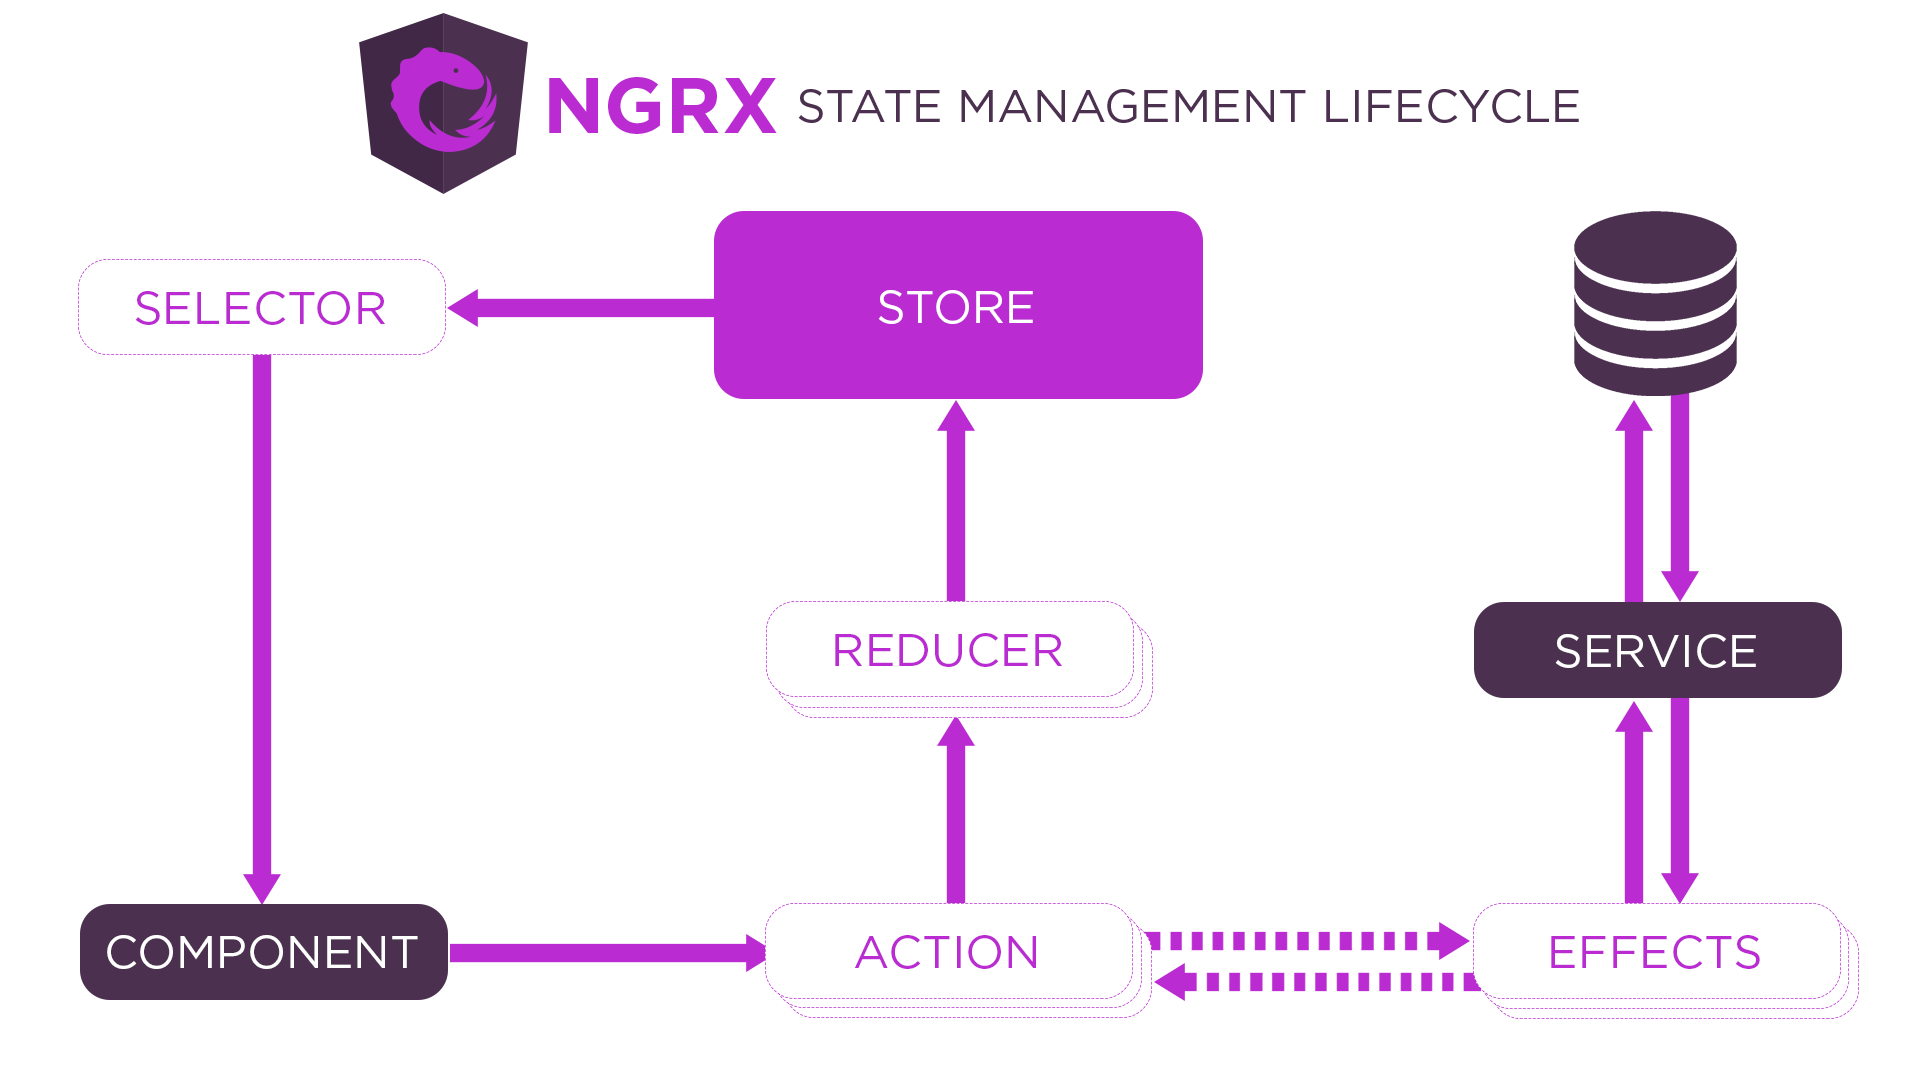
\includegraphics[width=\textwidth]{obrazky-figures/ngrx-lifecycle.png}
	\caption{Životní cyklus správy stavu s využitím knihovny NgRx. @todo popsat uzly \emph{Převzato z~\cite{bib:ngrx-lifecycle}}.}
\end{figure}
\blindtext

\subsubsection{DevExtreme}
DevExtreme je balík komponent určený pro tvorbu responzivních webových aplikací. Je k dispozici pro knihovny jQuery, Konockout, AngularJS, Angular, Vue, React, ASP.NET MVC 5 a ASP.NET Core.  
\blindtext

\section{REST}
\blindtext[2]

\section{JSON Web Token}
\emph{Tato podkapitola vychází z~\cite{bib:jwt}}

JSON Web Token (zkráceně JWT) je otevřený standard\footnote{RFC 7519: \url{https://tools.ietf.org/html/rfc7519}} zajišťující zabezpečenou výměnu informací mezi dvěma stranami. Jedná se o objekt typu JSON (JavaScript Object Notation), který se skládá ze tří částí oddělených tečkou. Jedná se o hlavičku, náklad a podpis.

Hlavička je objekt typu JSON, zakódovaný pomocí kódovaní Base64Url\footnote{Kódování reprezentující binární data pomocí tisknutelných znaků~\cite{bib:base64}}, který nese informaci o typu žetonu a použitém algoritmu digitálního podpisu. 

Náklad je stejně jako hlavička objekt typu JSON zakódovaný pomocí Base64Url. Tentokrát jsou však jeho obsahem tvrzení (angl. \emph{claim}). Ty nesou přenášené informace, které je třeba předávat zabezpečené. Nejčastěji se jedná o informace o uživateli.

Podpis zaručuje, že zpráva při přenosu nebyla pozměněna. Podpis může být také využit pro ověření identity odesílatele. Podpis je vytvořen spojením řetězců dvou předchozích částí, mezi které je vložena tečka. Na konec toho řetězce je dále připojen tajný řetězec. Výsledný řetězec je poté zašifrován algoritmem uvedeným v hlavičce. 

V praxi se lze s touto metodou autentizace setkat například na stránkách, které umožňují přihlásit se pomocí účtu u společnosti Google~\cite{bib:google-jwt}. V takovém případě se jedná o výměnu informací mezi třemi stranami. Posloupnost akcí pro získání žetonu v této situaci a jeho následné použití lze vidět na obrázku~\ref{img:jwt}.

\begin{figure}[H]
    \label{img:jwt}
	\centering
	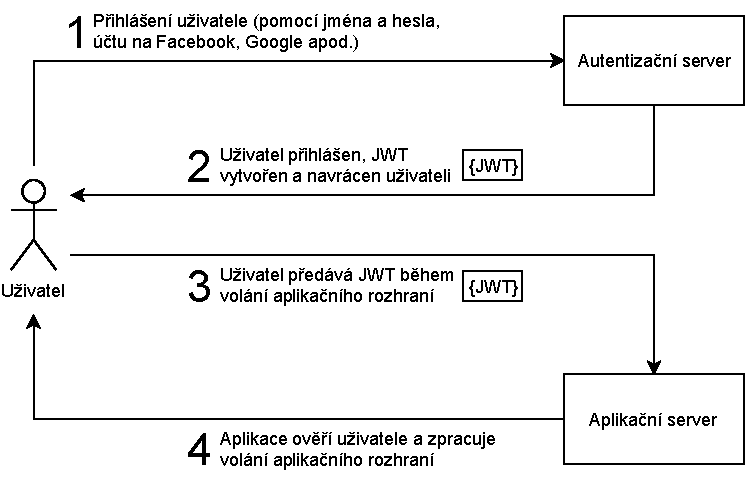
\includegraphics[width=0.9\textwidth]{obrazky-figures/jwt.pdf}
	\caption{Diagram znázorňující případ užití standardu JWT.}
\end{figure}

\section{ASP.NET Core}
ASP.NET Core je platforma společnosti Microsoft určena pro tvorbu webových aplikací. Jedná se o rozšíření populární platformy .NET určené především pro programovací jazyk C\#, taktéž vyvinutým společností Microsoft.

Přestože tato společnost stojí za dnes nejpopulárnějším operačním systémem Windows, je platformu ASP.NET Core možné provozovat i na jiných operačních systémech. Vydání první verze této platformy proběhlo v roce 2016~\cite{bib:asp-release}, dříve bylo možné platformu využít pouze na operačním systému Windows, tyto dřívější verze nesly název pouze ASP.NET bez označení Core~\cite{bib:asp-what-is}.

\blindtext

\section{PostgreSQL}
PostgreSQL\footnote{PostgreSQL: \url{https://www.postgresql.org}} je objektově-relační databázový systém s historií do roku 1986. Jedná se o vysoce přizpůsobitelné rozšíření jazyka SQL~\cite{bib:postgre}.
\blindtext



% ======================================================================
\chapter{Návrh aplikace}
Před samotnou implementací aplikace bylo nejprve nutné promyslet návrh tvořené aplikace. Zejména pak rozdělení aplikace do jednotlivých částí, určit jejich role v celkovém fungování systému a zmapovat interakci mezi těmito částmi. Některá rozhodnutí ohledně směru vývoje byly provedeny mnou samotným, některá ve spolupráci s konzultantem této bakalářské práce a jiná byla nařízena přímo vedením společnosti SEACOMP s.r.o.

Dále bylo třeba vytvořit návrh databáze, kde budou uložena data a také připravit grafický návrh. Mimo jiné bylo třeba zanalyzovat existující aplikační rozhraní a připravit jeho rozšíření. 
Právě těmto zmíněným oblastem se věnuje tato kapitola.




\section{Schéma systému}
Schéma aplikace je vidět na snímku~\ref{img:scheme}. Jsou zde znázorněny tři její hlavní části -- databáze, serverová část neboli SSBLite a v neposlední řadě webový klient Kanban. U každé z těchto částí je na snímku uvedena také její nejpodstatnější technologie. Dále zde lze pozorovat vzájemné interakce těchto části. Na pravé straně obrázku lze vidět dvě role uživatelů a také jejich interakci s aplikací.

\begin{figure}[H]
    \label{img:scheme}
	\centering
	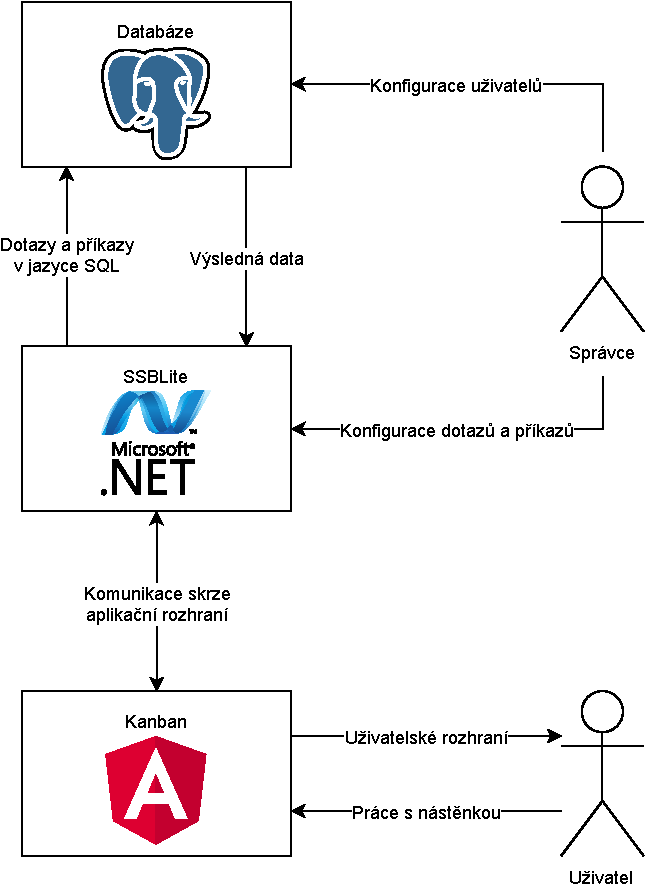
\includegraphics[width=0.8\textwidth]{obrazky-figures/app-scheme.pdf}
	\caption{Schéma vzájemných interakcí jednotlivých částí aplikace, jejich technologií a možnostech různých rolí uživatelů.}
\end{figure}

V tomto schématu se může jevit podivuhodná konfigurace uživatelů správcem přímo v databázi. V reálném prostředí, kde bude aplikace SSBLite nahrazena plnohodnotnou aplikací SSB, bude konfigurace probíhat již přímo v aplikaci SSB za pomocí uživatelského rozhraní. Nicméně pro účely této bakalářské práce postačí konfigurace tímto náhradním způsobem. Vzhledem k pozdějšímu nahrazení aplikace SSBLite by implementace této funkcionality byla bezpředmětná.

V práci taktéž není zakomponovaná správa samotných nástěnek. V současné aplikaci SSB totiž nástěnka odpovídá právě jednomu týmu uživatelů. Pro vytvoření nové nástěnky je tudíž nutné vytvořit celý nový tým. Z důvodů zachování tohoto chování a předcházení zbytečné dvojí implementace je pro vytvoření nebo odstranění nástěnky či přiřazení přístupu uživatelům k nástěnce nutné upravit data přímo v databázi. Tato funkcionalita bude taktéž vyřešena integrací do stávající aplikace.

\section{Entitně-vztahový diagram}\label{sec:erd}
Data aplikace jsou uložena v relační databázi. Systém SSB a tedy i SSBLite využívají databázový systém PostgreSQL. Data jsou uložena v jednotlivých tabulkách, které lze reprezentovat entitně-vztahovým diagramem znázorněným na obrázku~\ref{img:erd}. Názvy tabulek i sloupců jsou dle konvence společnosti v anglickém jazyce. Tabulky ve většině případu reprezentující entity (například nástěnky, karty nebo štítky), výjimku tvoří pouze propojovací tabulky, které reprezentují vztah M:N. Ty lze poznat podle číslovky 2 v názvu tabulky. Před a za touto číslovkou se pak nachází názvy entit, které ve vztahu figurují.

\begin{figure}[H]
	\centering
	\label{img:erd}
	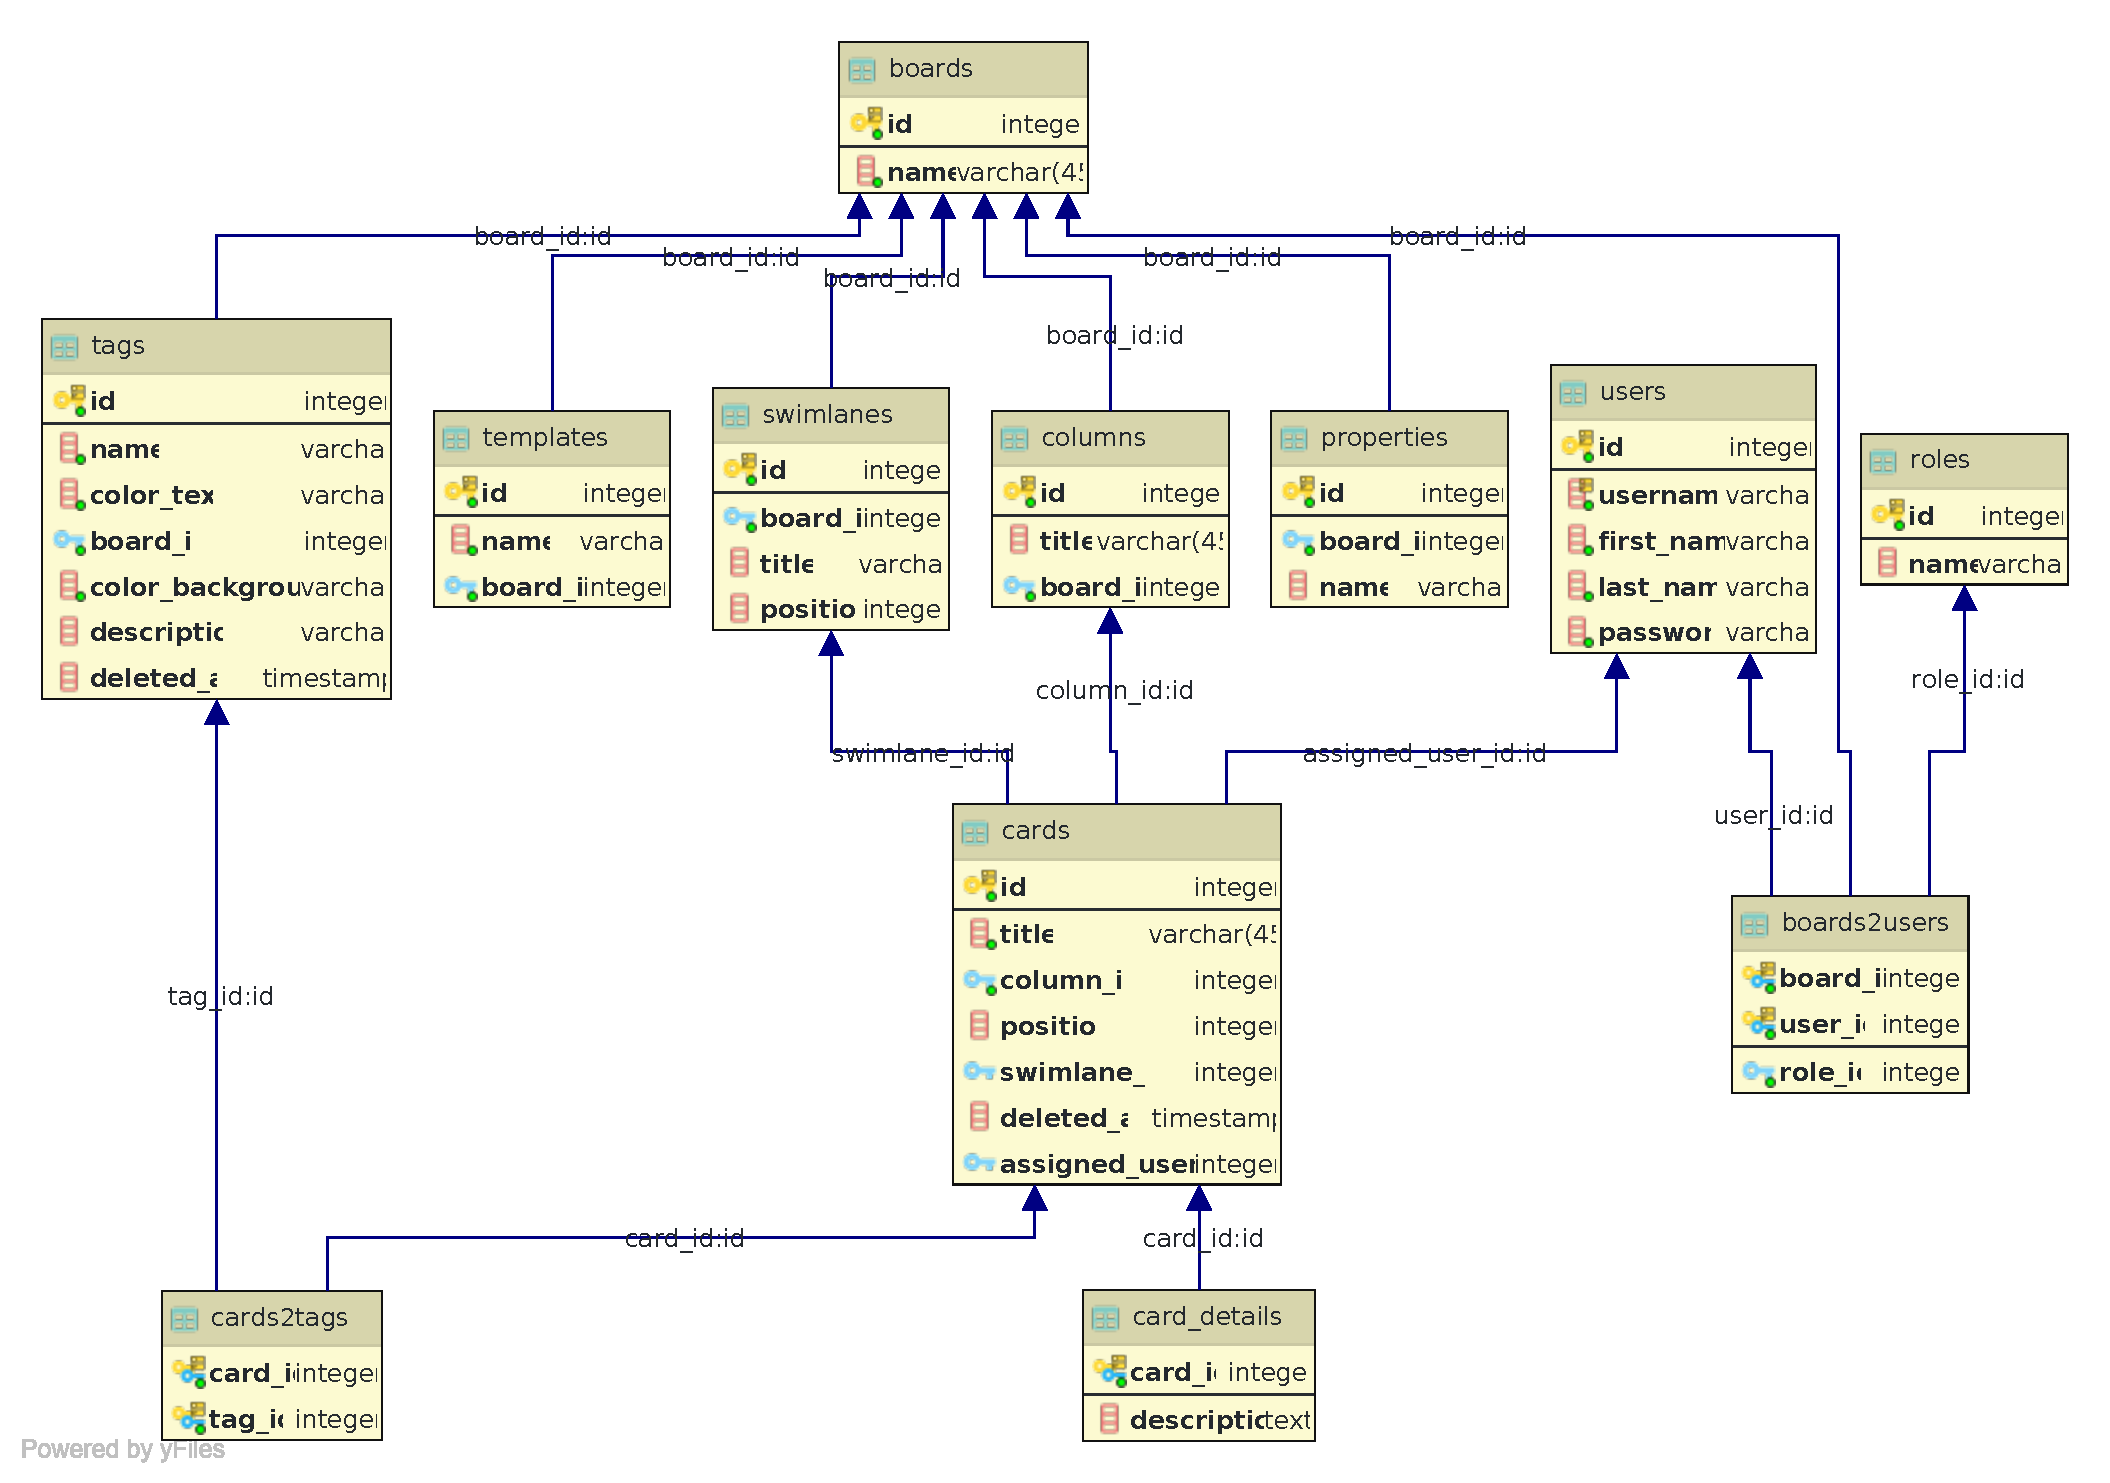
\includegraphics[width=\textwidth]{obrazky-figures/erd.pdf}
	% @todo Konverze z svg do pdf to nejak rozbila
	\caption{Entitně vztahový diagram reprezentující relační databázi aplikace.}
\end{figure}


\section{Grafický návrh}
Prvotní verze aplikace, která vznikla řešením této bakalářské práce bude využita pouze pro interní účely společnosti. Z tohoto důvodu nebyl při zadání práce kladen příliš velký důraz na estetickou stránku aplikace. Jedním z požadavků v tomto směru však bylo, aby aplikace co nejvíce využívala grafický styl knihovny DevExtreme. Další požadavek zněl, aby byly v aplikaci použity barvy loga společnosti SEACOMP s.r.o.

Ve všech částech aplikace je přítomna hlavička. Na levé straně je vždy obsaženo logo společnosti a na pravé straně se nachází informace o přihlášeném uživateli a akce jako jeho odhlášení. Po vzoru oficiální webové stránky společnosti\footnote{Webové stránky společnosti SEACOMP s.r.o.: \url{https://seacomp.cz}} hlavičku a obsah stránky dělí horizontální linka oranžové barvy, která je použita v samotném logu společnosti.

Co se grafického návrhu týče, nejrozsáhlejší část aplikace je jistě samotná nástěnka. Původní návrh je vyobrazen na snímku~\ref{img:design-kanban}. Z důvodu co největší maximalizace počtu zobrazených karet se nástěnka rozpíná po celé šířce i výšce stránky s výjimkou hlavičky a nástrojové lišty.

Ze stejného důvodu je menu ve výchozím stavu skryto a lze ho otevřít pomocí tlačítka na levé straně nástrojové lišty. Lišta dále obsahuje název právě otevřené nástěnky a po pravé straně pak vyhledávací pole.

Položky v menu i samotný detail karet se zobrazuje v modálním okně. Uživatel se tak například i při zobrazení detailu karty stále nachází na nástěnce a může se vrátit na její přehled téměř zcela bez prodlení na rozdíl od stávající aplikace využívané ve společnosti zadavatele, kde je pro zobrazení všech detailů nutné přejít na novou stránku a následný návrat na přehled je vzhledem k počtu zobrazených úkolu velmi pomalý.

Některé akce jako například odstranění karty lze provést podobně jako v desktopových aplikací pomocí kliknutí pravým tlačítkem myší na danou entitu. V případě dotykových obrazovek je kliknutí pravého tlačítka substituováno dlouhým stiskem. 

\begin{figure}[H]
	\centering
	\label{img:design-kanban}
	
\includegraphics[width=\textwidth]{obrazky-figures/placeholder.pdf}
	\caption{Grafický návrh části aplikace, kde je zobrazena nástěnka kanban, vytvořený pomocí nástroje MockFlow\footnote{MockFlow: \url{https://mockflow.com}}.}
\end{figure}

Další části aplikace jsou z pohledu uživatelského rozhraní velmi triviální, a proto pro jejich tvorbu návrh nebyl nevytvořen.


\section{Aplikační rozhraní}\label{sec:api}
Komunikace mezi klientskou částí aplikace a částí serverovou probíhá za pomoci aplikačního rozhraní REST. Zprávy tohoto rozhraní využívají formát JSON a mají přesně definovaný obsah.
Vzhledem k budoucí integraci mnou tvořené aplikace do již existující aplikace SSB4Web bylo nutné zachovat v obou těchto aplikacích jednotnou podobu rozhraní.

Vzhledem k zaměření mé aplikace nebylo třeba využít všechny možnosti existujícího rozhraní. Při práci byly z původního rozhraní použity pouze dva koncové body a to \texttt{SSBQuery/GetData}, umožňující dotazovat se na data uložena v databázi, a \sloppy\texttt{SSBMethod/ExecuteMethod}, spouštějící uložené procedury či příkazy. Toto rozhraní však bylo nutné rozšířit o možnost autentizace uživatele. Původní koncové body v tomto případě nebylo možné využít, protože pouze propagují dotazy databázi, kdežto pro autentizaci je třeba požadavek zpracovat přímo v aplikaci SSBLite. Z tohoto důvodu byl přidán nový koncový bod \sloppy\texttt{SSBAuthentication/VerifyCredentials}.

Obě části aplikace -- jak Kanban, tak SSBLite -- využívají stejné datové objekty, díky tomu je možné mezi těmito dvěma částmi jednoduše přenášet data. Obsahem požadavku pro získání dat je například objekt \texttt{SSBQueryRequestDTO}, ten s sebou nese jednak název konkrétního před-připraveného dotazu pod klíčem \texttt{queryName} a dále pod klíčem \texttt{filters} může obsahovat i další objekt typu \texttt{SSBFilterDTO}. Ten se zase skládá z objektu \texttt{ssbIFilterOperator}, skrytým pod stejnojmenným klíčem, a dále z pole objektů \texttt{SSBFilterTermDTO} označeným klíčem \texttt{filterItems}. Objekty v tomto poli obsahují tři hodnoty. Pod klíčem \texttt{m\_filterOperator} lze opět pozorovat objekt \texttt{ssbIFilterOperator}. Ve skutečnosti se jedná pouze o výčet logických operátorů, které jsou později použity pro bezpečné sestavení dotazu na databázi. Další dvě hodnoty nesou název sloupce v databázi a pole hodnot použitých v dotazu.

Konkrétní dotaz na získání karet s použitím filtru nástěnky tak může vypadat následovně:

\begin{verbatim}
{
  "queryName": "getCards",
  "limit": 0,
  "onlyVisibleColumns": true,
  "offset": 0,
  "filter":
    {
      "ssbIFilterOperator": 0,
      "filterItems":
        [
          {
            "m_filterOperator": 0,
            "m_column": "col.board_id",
            "m_values": [1] ¨
          }
        ]
    }
}
\end{verbatim}

Nevýhoda této podoby aplikačního rozhraní je však v nemožnosti provést více dotazů na databázi pomocí jednoho asynchronního volání. Například při prvotním načtení nástěnky je tak nutné odeslat vícero asynchronních požadavků najednou.

Tento nedostatek je způsoben tím, že je původní návrh rozhraní je zaměřen hlavně na zobrazení tabulek ve vztahu hlavní--podrobné (angl. \emph{master--detail}), kde k těmto situacím dochází minimálně. Zadavateli tématu diplomové práce bylo představeno několik alternativních řešení, nicméně bylo rozhodnuto pro zachování původního návrhu a setrvání v odesílání několika požadavků současně. 

% ======================================================================
\chapter{Implementace aplikace}
Předmětem této kapitoly je popis vlastní implementace webové aplikace typu Kanban, jejíž vytvoření bylo cílem této bakalářské práce. V úvodu je popsaná klientská část aplikace, ke které uživatel přistupuje pomocí internetového prohlížeče. Další část kapitoly je věnována implementaci serverové části aplikace, s kterou uživatel přichází do styku pouze skrze aplikační rozhraní, které již bylo přiblíženo v kapitole~\ref{sec:api}. Závěr kapitoly je pak zaměřen na databázovou vrstvu aplikace, kde jsou uchovávány uživatelská a jiná data.



\section{Klientská část}
Klientskou částí aplikace je jednostránková webová aplikace vytvořená za pomocí rámce Angular. Základním stavebním kamenem toho rámce jsou bez pochyby komponenty. Právě ty jsou hlavním tématem této podkapitoly. Dále jsou zde zmíněny i jiné zajímavé části implementace klientské části. Obsah jednotlivých stránek je sestaven kombinací vlastních komponent, které jsou podrobněji popsané v této kapitole, a také před-připravených komponent knihovny DevExtreme. Rozeznat jejich původ lze pomocí předpony \texttt{app-} v případě vlastních komponent a pomocí předpony \texttt{dx-} v případě komponent z knihovny DevExtreme.


\subsection{Struktura adresáře}
Adresář, ve kterém se nachází zdrojové kódy aplikace je kvůli využití rámce Angular poměrně rozsáhlá. Některé jeho části, které stojí za zmínku jsou popsány v této podkapitole. Zajímavé části nejvyšší úroveň adresáře aplikace vypadají následovně:

\begin{itemize}
  \item \texttt{node\_modules} -- Zdrojové kódy knihoven třetích stran
  \item \texttt{src} -- Zdrojové kódy aplikace
  \begin{itemize}
    \item \texttt{app} -- Adresář obsahující zdrojové kódy aplikace v jazyce TypeScript
     \item \texttt{assets} -- Adresář obsahující statický obsah stránky jako například globální kaskádové styly a obrázky
     \item \texttt{index.html} -- Hlavní stránka aplikace
  \end{itemize}
  \item \texttt{angular.json} -- Konfigurace rámce Angular
  \item \texttt{package.json} -- Konfigurace závislostí na knihovnách třetích stran
\end{itemize}

Nejdůležitějším z výše uvedených adresářů je jednoznačně adresář \texttt{app}. Pro lepší přehlednost je jeho obsah uveden zvlášť níže:

\begin{itemize}
  \item \texttt{} -- 
  \item \texttt{} --
\end{itemize}


\subsection{Základní struktura stránky}
Ať už se uživatel aktuálně nachází na libovolné části aplikace, základní struktura právě zobrazené stránky se bude tvořit ze stejných prvků. Základ celé komponenty je element \texttt{<app-root>}. Tento prvek je také kromě referencí na soubory obsahující zdrojové kódy jazyka JavaScript to jediné, co se v obsahu stránky zobrazí v případě, že internetový prohlížeč jazyk JavaScript nepodporuje či dokonce blokuje. 

V případě, že je interpret jazyka JavaScript dostupný, vzniknou uvnitř tohoto elementu další elementy. Vždy je přítomna komponenta \texttt{<app-header>} a \texttt{<router-outlet>}. První z komponent obsahuje hlavičku s logem společnosti SEACOMP s.r.o., která je vždy vidět ve vrchní části aplikace. Součástí hlavičky je také možnost odhlášení uživatele, za předpokladu že je právě přihlášen. Tato komponenta je vyfocena na snímku~\ref{img:comp-header}.


\begin{figure}[H]
	\centering
	\label{img:comp-header}
	
\includegraphics[width=\textwidth]{obrazky-figures/comp-header.png}
	\caption{Ukázka komponenty hlavičky neboli \texttt{<app-header>} s právě přihlášeným uživatelem.}
\end{figure}

Druhá z komponent ve skutečnosti nemá žádný reálný obsah. Představuje však nedílnou součást aplikace, jelikož se stará právě o chování aplikace jako jednostránkové. Na základě aktuální cesty obměňuje komponentu, která v hierarchii uzlů HTML představuje dalšího sourozence. Z počátku se tak lze na tomto místě potkat s komponentou \texttt{<app-login>}, následně \texttt{<app-dashboard>} a poté \texttt{<app-board>}. Současně s obměnou těchto komponent je také změněna adresa aktuální stránky v adresním řádku internetového prohlížeče. Navenek se tedy může zdát, že uživatel skutečně přechází z jedné stránky na druhou. Ve skutečnosti se však nachází stále na stejné stránce, pouze je překreslována část jejího obsahu.

Cesty a jim odpovídající komponenty jsou definované v souboru \texttt{app-routing.module.ts}. U každé cesty je také možno nastavit ochranné služby. Jedná se o třídy implementující rozhraní \texttt{CanActivate}, které ve stejnojmenné metodě vrací logickou hodnotu. Pokud jedna z těchto služeb vrátí hodnotu nepravdy, je přístup uživatel k této cestě zamítnut. Tuto funkcionalitu v aplikaci využívám na ověření, zda je uživatel přihlášen. Výjimku tvoří pouze stránka s přihlášením, ke které lze přistoupit v přesné opačné situaci a to když uživatel zatím není přihlášen. Jedná se o třídy \texttt{AuthenticationGuardService} a \texttt{GuestGuardService}.


\subsection{Nástěnka}
Stránka s nástěnkou je bezesporu nejkomplexnější částí aplikace. Základní komponentou je v tomto případě \texttt{<app-board>}, jejím úkolem je mimo jiné také prvotní načtení všech dat z databáze, které se dané nástěnky týkají. Jedná se například o sloupce, plavecké dráhy, karty, štítky a další entity. Celkový přehled důležitých komponent této stránky je uveden na snímku~\ref{img:comp-board-scheme}.

Na nejvyšší úrovni této stránky se nachází několik komponent knihovny DevExtreme. Nejvýše položená komponenta je \texttt{<dx-toolbar>}, která obsahuje tlačítko pro zobrazení či skrytí menu, název nástěnky a vyhledávací pole. Hned pod ní se nachází komponenta \texttt{<dx-drawer>}, ta slouží k zobrazení nabídky menu. Jistou zvláštností je, že celá zbylá část stránky se nachází uvnitř této komponenty, nicméně použitá knihovna vyžaduje takovýto přístup.

Obsahem zmíněné komponenty je další komponenta knihovny DevExtreme a to \texttt{<dx-scroll-view>}. V tomto případě nahrazuje nativní posuvné lišty internetového prohlížeče a to jak vertikální, tak i horizontální. Tím je zajištěno jednotné chování i vzhled těchto lišt napříč různými prohlížeči.

\begin{figure}[H]
	\centering
	\label{img:comp-board-scheme}
	
\includegraphics[width=\textwidth]{obrazky-figures/placeholder.pdf}
	\caption{Ukázka stránky s nástěnkou se zvýrazněním jednotlivých komponent.}
\end{figure}

\subsubsection*{Plavecké dráhy}

Uvnitř této komponenty se již nacházejí vlastní komponenty specifické pro nástěnku Kanban. V hiearchii se nejvýše nachází komponenty \texttt{<app-board-swimlane>}, kde jedna vždy odpovídá jedné plavecké dráze. Plavecké dráhy se skládají ze samotného záhlaví dráhy a dále z obsahu. Ten lze pomocí kliknutí na záhlaví zobrazit či skrýt, což je užitečná funkcionalita v případě, že je těchto drah využito mnoho. 

\subsubsection*{Sloupce}

Uvnitř každé plavecké dráhy se pak pro každý sloupec nástěnky nachází právě jedna komponenta typu \texttt{<app-board-column>}. Ta sdružuje karty, naležící danému sloupic a plavecké dráze. Sloupec opět využívá komponentu \texttt{<dx-scroll-view}, která s kombinací s fixní výškou sloupce zajišťuje, že nadměrné hromadění karet v jednom sloupci neovlivňuje okolní sloupce, jako tomu je v současnosti u původní aplikace.

Obsahem sloupců je také komponenta \texttt{<dx-sortable>}, která umožňuje přesun karet mezi jednotlivými sloupci a plaveckými drahami. Jedna z metod této komponenty však byla přepsány. Jedná se o metodu, který je spuštěna po přesunu karty. Ta kromě provedení samotné změny pozice také o této změně informuje serverovou část aplikace. 

\subsection{Karta}

\blindtext

\subsubsection*{Detail karty}
\blindtext


\subsection{Nastavení}
Ačkoliv některá nastavení se v současné aplikaci provádí editací dat v databázi, existuje i několik případů, kdy se nastavení nachází přímo v aplikaci a je realizováno pomocí uživatelského rozhraní. Implementace takových nastavení je popsána v této podkapitole.

\subsubsection*{Nastavení štítků}
Modální okno s nastavením štítků cíleně porušuje jeden z pravidel principu Flux. Uchovává totiž lokální kopii sdílených dat uložených ve skladu. Tento přístup jsem zvolil z jednoho prostého důvodu a to aby se v případě zahození změn nemusel stav štítků napříč celou aplikací změnit. Místo toho jsem se přiklonil k opačnému řešení. Při úpravě štítků uživatel pracuje pouze s kopií sdílených dat. Jeho změny se tak neprojevují v jiných komponentách. V případě zahození změn při zavření dialogu tudíž není nutné provést vůbec žádnou akci. 

\subsubsection*{Sdílené komponenty}
Některá nastavení jsou si vzájemně velice podobná. Z toho důvodu bylo nastavení rozděleno do několika menších komponent a několik z nich tak lze použít například jak v nastavení sloupců, tak i v nastavení plaveckých drah.

Hierarchie těchto komponent je vyobrazena na snímku~\ref{img:settings-dia}. Detailní popis jednotlivých komponent a jejich funkcí je popsán dále v této podkapitole.

\begin{figure}[H]
	\centering
	\label{img:settings-dia}
	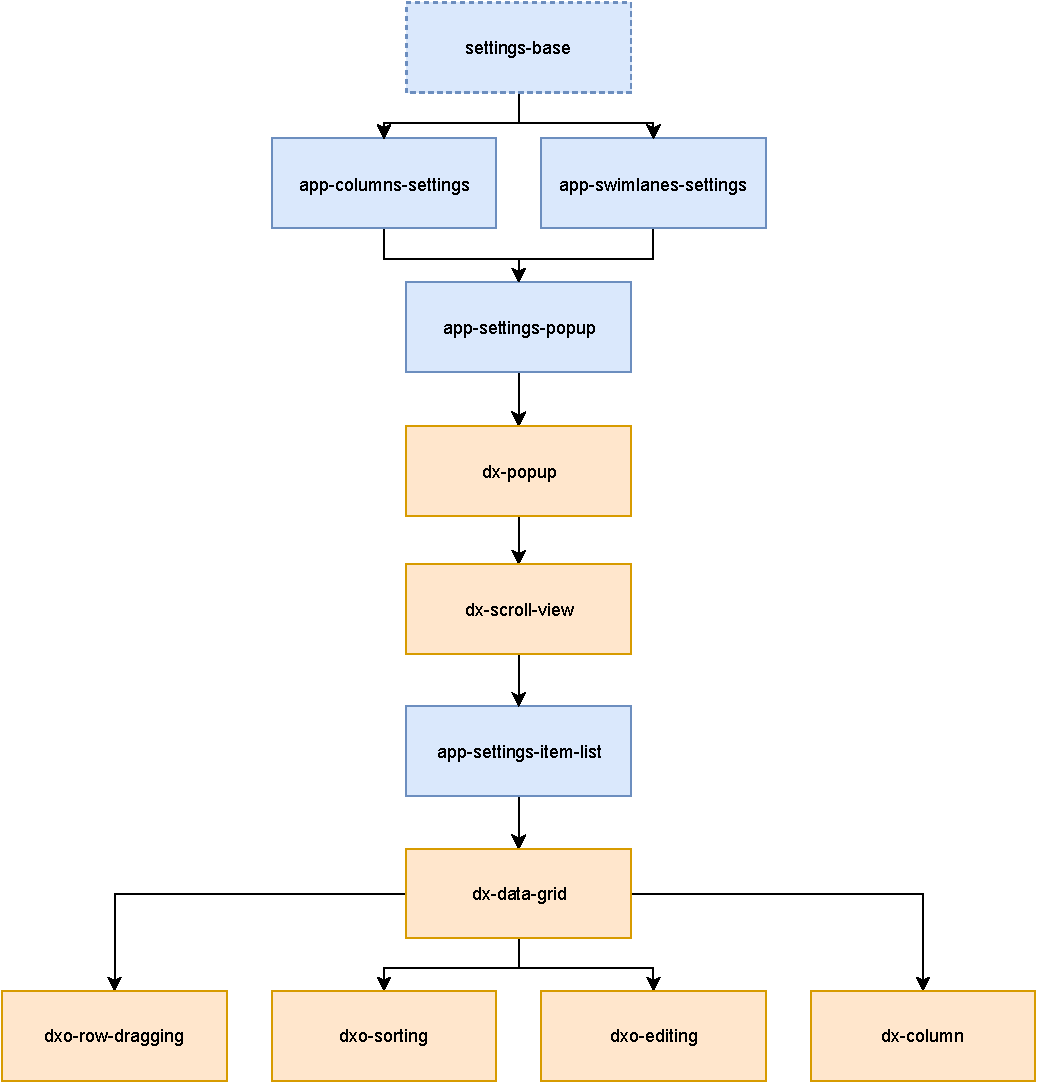
\includegraphics[width=\textwidth]{obrazky-figures/settings-diagram.pdf}
	\caption{Diagram znázorňující hierarchii jednotlivých komponent a tříd využitým pro realizování modálních oken pro nastavení nástěnky. Vlastní části řešení jsou označeny modrou barvou a komponenty knihovny DevExtreme jsou označeny oranžově. Komponenty jsou znázorněny plným ohraničením a abstraktní třída čárkovaným.}
\end{figure}


\subsubsection*{Třída SettingsBase}
Jedná se o abstraktní třídu, z které dědí konkrétní komponenty pro jednotlivá nastavení jako například \texttt{<app-columns-settings>} pro nastavení sloupců nebo  \texttt{<app-swimlanes-settings>} pro nastavení řádků. Hlavním účelem této abstraktní třídy je sjednotit způsob propagace otevření modálního okna.


\subsubsection*{Komponenta app-settings-popup}
Veškerá nastavení nástěnky probíhají za pomoci modálních oken. Samotné grafické zobrazení oken je realizováno pomocí komponenty knihovny DevExtreme a to konkrétně \texttt{<dx-popup>}. Tato komponenta je však rozšířena o varování při pokusu o zavření okna s neuloženými daty. Zmíněné chování je součástí implementace komponenty \texttt{<app-settings-popup>}.


\subsubsection*{Komponenta app-settings-item-list}
Další opakovaně vyskytující částí nastavení je datová mřížka (angl. \emph{data grid}). Tato mřížka by se dala označit jako rozšířená tabulka s akcemi umožňující manipulaci a editaci dat. Stejně jako u předchozí komponenty je pro grafické zobrazení této mřížky využita knihovna DevExtreme a její komponenta \texttt{<dx-data-grid>}. Komponenta mimo pouhé zobrazení umožňuje i samotnou práci s daty, nicméně během implementace byl zjištěn nedostatek při současném využití řazení dle sloupce a možnosti měnit pořadí řádků.

Při úpravě hodnot se mění pouze lokální kopie dat, kterou si komponenta uchovává. Tyto hodnoty se v původním zdroji dat projeví až po uložení. Nicméně řazení probíhá podle zdrojových dat a ne podle dat lokálních.

Především kvůli vlastní implementaci změny pořadí byla vytvořena komponenta \texttt{<app-settings-item-list>}. Mimo jiné slouží pro unifikaci nastavení samotné datové mřížky, které je realizováno pomocí vnořených elementů uvnitř komponenty \texttt{<dx-data-grid>}. Dále však obsahuje celou řadu metod, které téměř kompletně mění standardní chování komponenty mřížky. Realizuje zejména změnu pořadí řádků a vlastní chování tlačítek pro přidání a mazání řádků, obnovení změn a jejich ukládání.

Změna pořadí dat tedy v mé implementaci mění hodnoty jak v lokální kopii dat uvnitř komponenty \texttt{<dx-data-grid>}, tak i v jejím datovém zdroji. Jelikož je nutné neuložené změny projevovat i v datovém zdroji, tak existuje i třetí kopie dat, kterou si uchovává komponenta \texttt{<app-settings-item-list>} pro případnou obnovu dat při zahození změn.

Tlačítko pro smazání záznamu celý řádek odstraní z mřížky. Původní chování byla pouze změna barvy. Tlačítko pro přidání nového záznamu bylo pozměněno opět z důvodu zachování možnosti změny pořadí řádků. Tlačítko uložení pak bylo nutné rozšířit z důvodu absence události uložení dat v komponentě \texttt{<dx-data-grid>}. Pro případ použití v této aplikaci nestačí změnit hodnoty v datovém zdroji, ale je nutné změny projevit i v databázi na serveru a právě tento požadavek je nyní odeslán pomocí tlačítka uložení. 


\subsection{Asynchronní požadavky}
Jak již bylo zmíněno v kapitole~\ref{sec:spa}, jednostránkové aplikace fungují hlavně díky asynchronním požadavkům. Ty jsou tedy samozřejmě nedílnou součástí i této aplikace.

Po přihlášení uživatele každý jeho asynchronní požadavek v hlavičce protokolu HTTP obsahuje žeton standardu JWT. O tuto funkci se stará třída \texttt{JwtInterceptor}, umístěná ve složce \texttt{interceptors}. Třída naslouchá všem odesílaným požadavkům protokolu HTTP a v případě, že je žeton již dostupný, je před samotným odesláním požadavku nejprve rozšířena hlavička tohoto požadavku. Do pole \texttt{Authorization} je vloženo slovo \texttt{Bearer} a za mezerou následuje samotný žeton.

Ve stejné složce lze také nalézt další třídu \texttt{ErrorInterceptor}, která obstarává oznámení uživateli v případě negativní odpovědi na odeslaný požadavek. Tato třída byla užitečná obzvláště během vývoje, jelikož chyby jazyka JavaScript se zobrazují v konzoli internetového prohlížeče, tudíž nejsou na první pohled zřetelné. Nicméně tato třída přináší užitek i pro koncové uživatele ve výsledné verzi aplikace.

V případě úspěšné odpovědi na asynchronní požadavek jsou data obsažená v této zprávě uložena do skladu dat. Tento proces je podrobněji vysvětlen v následující kapitole.

O samotné vytvoření zmíněných požadavků se starají služby \texttt{AuthenticationService}, \texttt{SSBMethodService} a \texttt{SSBQueryService}. Jejich chování lze částečně konfigurovat v souborech s prostředím umístěných ve složce \texttt{environments}.


\subsection{Centrální datový sklad}
Data sdílena mezi více komponentami jsou uložena v centrálním skladu, který je realizován pomocí knihovny NgRx. Při implementaci byl kladen důraz na co nejmenší zanořování dat, která jsou v tomto skladu přítomna. Každé sdílené entitě (např. nástěnkám, uživatelům, štítkům) tedy odpovídá právě jeden objekt v první úrovni zanoření.

Každý z těchto objektů je pak tvořen dalšími třemi hodnotami. Klíč \texttt{loading} obsahuje logickou hodnotu, která indikuje, zda se data právě načítají. Tato hodnota je kladná v období mezi odesláním asynchronního požadavku a přijmutím odpovědi od serveru. Uživateli tak může být dočasně skryt obsah části stránky, který je závislý na stále ještě nedostupných datech. V případě kladné odpovědi jsou přijatá data převedena do vhodného tvaru a poté uložena jako pole či objekt do hodnoty označené klíčem \texttt{data}. V případě neúspěchu dotazu je pak chyba uložena do hodnoty pod klíčem \texttt{error}.

O zmíněné převedení formátu se stará třída \texttt{SSBQueryDataResultParser}. Ta převádí nevhodný tvar dat přenášených pomocí aplikačního rozhraní, kde je informace o sloupcích a datech rozdělena do dvou polí. Metoda této třídy z těchto dvou polí vytvoří jedno pole obsahující objekty, ve kterých jsou již názvy sloupců a jejich hodnoty v podobě jaká je u objektů typu JSON obvyklá.

Ani tato podoba dat však není finální. Výstupem zmíněné metody jsou totiž generické objekty. Pro veškeré přenášené entity však v aplikaci existuje odpovídající třída ve složce \texttt{models}. Generické objekty sice v aplikaci ve většině případů fungují, ale chybí jím specifické metody. V případě modelu uživatele lze například využít virtuální atribut \texttt{fullName}, který je ve skutečnosti pouze složenina dvou jiných atributů. Tento atribut by tedy v případě generického objektu dostupný nebyl. 
To je důvodem proč je využita funkce \texttt{plainToClass} knihovny \texttt{class-transformer}\footnote{Repozitář knihovny class-transformer: \url{https://github.com/typestack/class-transformer}}, která data dále převede do finální podoby.

Samotné ukládání přijatých dat a změnu obsahu skladu se zase starají reduktory (angl. \emph{reducers}), které využívají zmíněnou třídu pro převod dat. 

Okamžitá vizuální odezva je však pro uživatele velmi důležitá. V některých případech je tak tedy nutné data ve skladu změnit dříve, než je přijata odpověď od serveru. Je tomu tak například u přesunu karty. Jistě by bylo pro uživatele velice nepříjemné, kdyby přesunul kartu na nové místo a ta se vzápětí ihned vrátila na svou původní pozici a až po nějaké době by akci potvrdil server a karta by se přesunula na místo, kam uživatel původně zamýšlel. Proto je v takových případech předpokládán úspěch akce a data ve skladu jsou ihned změněna. I tuto práci obstarává reduktor.

Pro lepší ilustraci je níže uveden snímek~\ref{img:ngrx-devtools}, který ilustruje část dat aplikace uložených právě v popisovaném centrálním skladu.

\begin{figure}[H]
	\centering
	\label{img:ngrx-devtools}
	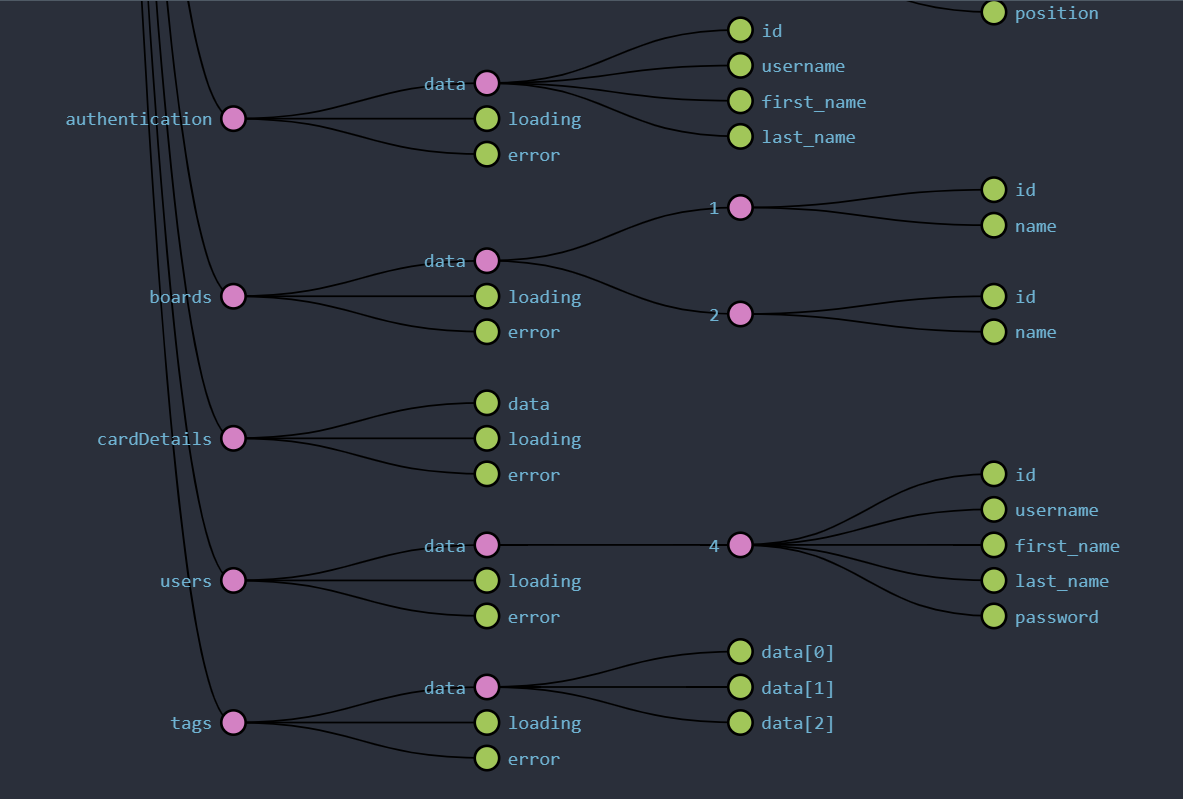
\includegraphics[width=\textwidth]{obrazky-figures/ngrx-chart.png}
	\caption{Vizualizace dat obsažených v centrálním datovém skladu. Snímek je pořízen z nástroje Redux DevTools\footnote{Redux DevTools: \url{https://chrome.google.com/webstore/detail/redux-devtools/lmhkpmbekcpmknklioeibfkpmmfibljd}}}
\end{figure}

Další dvě nedílné součásti knihovny NgRx jsou efekty a akce. Jejich účel byl již popsán v kapitole~\ref{sec:ngrx}. Každé ze sdílených entit naleží vlastní trojce těchto součástí knihovny. Obsah asynchronních požadavků je sestaven přímo v souboru s efekty, odkud jsou následně volány služby, které mají na starost tyto požadavky odeslat aplikaci SSBLite.



% ======================================================================
\section{Serverová část}
Z důvodu zachování firemního tajemství klientská část mé práce nekomunikuje přímo se systémem SSB, ale pouze se zjednodušenou verzí zvanou SSBLite, kterou jsem vytvořil v rámci řešení této bakalářské práce. Jedná se o webový server vytvořený s použitím systému ASP.NET. Server zpracovává požadavky aplikačního rozhraní REST na základě kterých sestrojuje a odesílá požadavky na databázi. Výsledky těchto požadavků jsou poté odeslány zpět klientovi ke zpracování a zobrazení uživateli.

Samotný webový server kromě autentizace uživatele neobsahuje žádnou aplikační logiku. Slouží pouze jako zprostředkovatel přístupu k databázi, ke které klient z důvodu bezpečnosti nesmí mít přímý přístup. Možné požadavky na databázi jsou předem definovány a uloženy v konfiguračních souborech. Díky tomu je možné v budoucnu upravit chování aplikace bez nutnosti přímého zásahu do zdrojového kódu serverové části aplikace. 


\subsection{Struktura adresáře}
V této podkapitole je popsán adesář obsahující zdrojové aplikace SSBLite. Některé nepodstatné soubory a adresáře nejsou v seznamu uvedeny. Jedná se o podobu adresáře bez vygenerovaných souborů, tak jako na přiloženém médiu. Po úspěšném překladu se vytvoří nové soubory uvnitř adresáře \texttt{bin}.

\begin{itemize}
  \item \texttt{Configurations/} -- Adresář obsahující konfigurační soubory metod a dotazů na databázi
  \item \texttt{Controllers/} -- Adresář obsahující řídící třídy
  \item \texttt{Enums/} -- Adresář obsahující objekty výčtů, používaných aplikačním rozhraním
  \item \texttt{Helpers/} -- Adresář obsahující třídu, která umožňuje přístup k tajnému klíči aplikačního rozhraní
  \item \texttt{Interfaces/} -- Adrsář s rozhraními
  \item \texttt{Models/} -- Adresář s třídami objektů modelů
  \begin{itemize}
    \item \texttt{Authentication/} -- Modely týkající se autentizace uživatele
    \item \texttt{Method/} -- Modely týkající se metod a příkazů databázi
    \item \texttt{Query/} -- Modely týkající se dotazů na databázi 
  \end{itemize}
  \item \texttt{Services/} -- Adresář se službami získávající data z databáze
  \item \texttt{appsettings.json} -- Soubor s konfigurací aplikace
  \item \texttt{Startup.cs} -- Soubor se spouštěcí třídou s další konfigurací
\end{itemize}


\subsection{Rozhraní Swagger}
V raných etapách vývoje, kdy ještě nebyla klientská a serverová část aplikace vzájemně propojena, byl pro testování vývoje používán rámec Swagger\footnote{Swagger: \url{https://swagger.io}}. Díky jeho využití byly možnosti a podoba aplikačního rozhraní přehledně uvedena na jednom místě, odkud bylo také možné jednitlivé požadavky odesílat.

Tento nástroj je ve výsledné aplikaci stále dostupný při překladu aplikace pro vývojové prostředí. Vzhledem k absenci jeho použití v pozdějších fázích vývoje však neobsahuje nejaktuálnější změny v aplikaci, i tak jej však lze využít zejména pro orientaci v aplikačním rozhraní. Ukázka části tohoto rozhraní je vidět na snímku~\ref{img:swagger}.

\begin{figure}[H]
	\centering
	\label{img:swagger}
	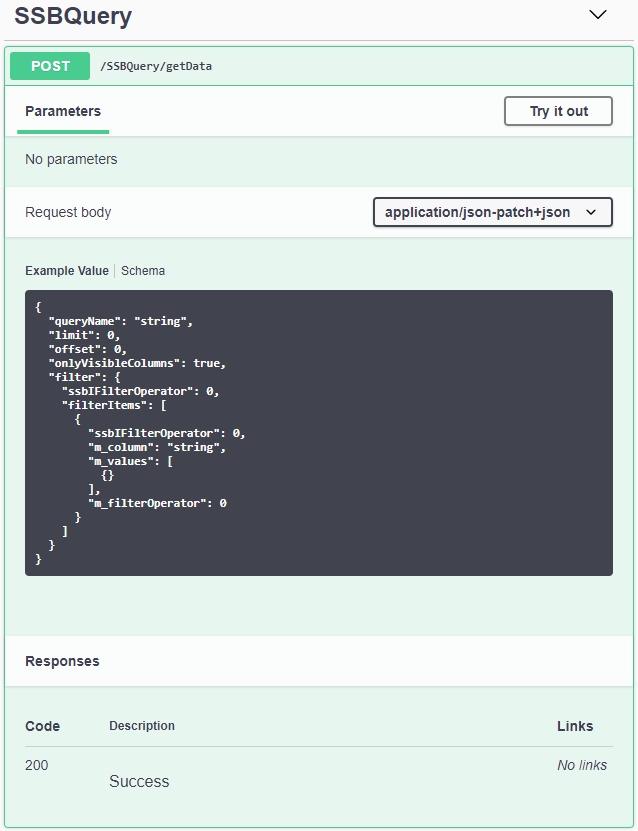
\includegraphics[width=\textwidth]{obrazky-figures/swagger.png}
	\caption{Popis části aplikačního rozhraní umožňující dotazovat se na data uložená v aplikaci znázorněný v uživatelském rozhraní rámce Swagger.}
\end{figure}

\subsection{Konfigurační soubory}
Konfigurační soubory využívají formát JSON a obsahují názvy jednotlivých požadavků a jejich znění. To však v mnoha případech přímo neobsahuje platný dotaz na databázi, ale obsažený dotaz je obohacen o klíčová slova, která umožňují přizpůsobení jeho znění pro aktuální potřebu klienta. Před samotným odesláním dotazu do databáze je nutné tyto klíčová slova zpracovat. Příkladem, využívajícím klíčové slovo \texttt{\{WHERE\}}, je následující dotaz:
\begin{verbatim}
{
    "name": "getCards",
    "content": "SELECT car.* FROM cards car JOIN columns col ON col.id = 
        car.column_id JOIN boards boa ON boa.id = col.board_id {WHERE}"
},
\end{verbatim}


\subsection{Zpracování požadavku GetData}
\blindtext


\subsection{Zpracování požadavku ExecuteMethod}
\blindtext


\subsection{Autentizace uživatele}
\blindtext



\section{Databázová vrstva}
Jak již bylo zmíněno, databáze využívá systém PostgreSQL. Ve většině podobných aplikací databáze slouží pouze pro úschovu dat. Nicméně kvůli univerzálnosti systému SSB je nutné v databázi uchovávat i aplikační logika. Toho je docíleno pomocí uložených procedur. Koncepce uložení dat v databázi byla zmíněna již v podkapitole~\ref{sec:erd}.

Jednodušší procedury jsou psány přímo v jazyce SQL a jedná se tak především o sekvenci vícero klasických příkazů, které lze spustit pomocí jednoho příkazu (spuštění uložené procedury). Tento přístup je využit například při vytvoření nového štítku, kdy je část dat uložena v tabulce \texttt{cards} a část v tabulce \texttt{card\_details}.
% @todo Overit jestli jsem to uz nezmenil

Pro komplexnější akce bylo však nutné využít jazyk PL/pgSQL\footnote{PL/pgSQL: \url{https://www.postgresql.org/docs/9.6/plpgsql.html}}. Ten umožňuje používat například funkce nebo podmínky.

Dle požadavku zadavatele práce názvy uložených procedur dodržují konvenci, kdy v první částí názvu je uvedena entita, které se daná operace týká a v druhé části je název akce. Lze se tedy setkat s názvy jako je \texttt{tags\_sync}, která synchronizuje štítky přiřazené dané kartě. 


\subsection{Synchronizace záznamů}
V aplikaci je několik situací kdy je třeba synchronizovat záznamy. Jedná se o tři akce s daty -- úprava a odstranění existujících záznamů a vytvoření nových. Tato situace nastává zejména při nastavování nástěnky. Konkrétně při nastavení sloupců, plaveckých drah, štítků a podobně. Tyto akce jsou provedeny pomoci uložených procedur \texttt{column\_sync}, \texttt{swimlane\_sync}, \texttt{tag\_sync}.

Uvnitř této procedury se však nachází pouze volání další uložené procedury a to jedné a té stejné pro všechny zmíněné procedury. Jedná se o proceduru \texttt{sync\_handler}, která umožňuje dynamicky provádět právě synchronizaci dat. Jejími parametry jsou jednak vstupní data původních procedur (identifikátor nástěnky a data k synchronizaci) a dále také specifikace nástěnky, kde jsou data uložena a sloupce, kterých se synchronizace týká.

Díky tomu je značně zredukována redundance kódu a v kombinaci s generickým komponentami klientské aplikace lze celý systém jednoduše rozšířit o nastavení dalších prvků.


\subsection{Autentizace požadavků}
\blindtext


\subsection{Ukládání historie}
\blindtext


% ======================================================================
\chapter{Testování a vyhodnocení}
\blindtext

Automatizované testování nebylo při práci využito. Bylo tak rozhodnuto po konzultaci jak s vedoucím tak i se zadavatelem práce. Pro ověření funkčnosti, bezpečnosti a dalších aspektů aplikačního rozhraní bylo využito manuální testování pomocí nástroje Postman\footnote{Postman: \url{https://www.postman.com}}, který slouží jako klient pro odesílání požadavků aplikačního rozhraní REST a zobrazení odpovědí na tyto požadavky.

\subsection{Uživatelské testování}
Testování na uživatelích probíhalo na @todo zaměstnancích společnosti SEACOMP s.r.o. Jednalo se jak o zástupce z řad vedoucích týmů, kteří v rámci své pozice pracují s nástěnkou kanban dennodenně a mají na starost i její konfiguraci, tak i o řadové programátory, kteří tento nástroj využívají zřídka a čistě jen z uživatelského pohledu.

Vzhledem k současné pandemii koronaviru bylo nutné využít pouze prostředky pro vzdálenou komunikaci. Testování tak bylo rozděleno do dvou částí. První část obnášela samotné vyzkoušení aplikace uživatelem. Druhá část byla realizována pomocí dotazníku.

\subsubsection{Testovací data}
Pro každého účastníka uživatelského testování byl vytvořen vlastní účet a k němu také separátní nástěnka se základními sloupci a plaveckými drahami. K nástěnce bylo přiřazeno dalších deset uživatelů. Obsahem nástěnky však byla pouze jediná karta. Uživatelé tak tedy začali téměř s netknutou nástěnkou. Tyto testovací data byla vytvořena pomocí databázové funkce \texttt{test\_table\_create}.

\subsubsection{Sledování chování uživatelů}
Uživatel nebyl dopředu s aplikací nijak seznámen, protože vzhledem k zaměření jeho povolání byl předpoklad, že se s podobným nástrojem v minulosti již setkal. 

Aplikace třetích stran umožňující zaznamenat pohyb myši a průchod aplikací bohužel nebylo možné využít, jelikož nedokázaly správně zpracovat kaskádové styly aplikace a výsledný záznam tak byl takřka nepoužitelný. Náhradní řešení tedy bylo sledování vybraných uživatelů pomocí sdílení obrazovky prostřednictvím aplikace Skype\footnote{Skype: \url{https://www.skype.com/cs/}}.

\subsubsection{Dotazník}
Po vyzkoušení aplikace každý z testovacích uživatelů obdržel odkaz na elektronický dotazník realizovaný pomocí online nástroje Formuláře Google\footnote{Formuláře Google: \url{https://www.google.com/intl/cs/forms/about/}}. Otázky dotazníku byly rozděleny do dvou skupin a jejich znění je uvedeno v příloze~\ref{sec:questionarre}.

První skupina obsahovala deset výroků na téma použitelnosti aplikace a respondent byl požádán o vybrání hodnoty na škále od jedné do pěti, zda s daným výrokem souhlasí či nesouhlasí. Znění těchto výroků vychází z překladu standardizovaného dotazníku zvaného Měřítko použitelnosti systému\footnote{Měřítko použitelnosti systém: \url{https://www.usability.gov/how-to-and-tools/methods/system-usability-scale.html}} (angl. \emph{System Usability Scale} neboli \emph{SUS}).

Druhá skupina obsahovala pět otevřených otázek zaměřených na silné a slabé stránky aplikace a její srovnání s původní aplikací, která se ve společnosti SEACOMP s.r.o. právě využívá.



\subsection{Vyhodnocení}
Vyhodnocení bylo rozděleno do tří částí. První se věnuje čistě jen samotnému dotazníku Měřítka použitelnosti systému. Další část se zabývá poznatky zjištěnými druhou částí dotazníku a sledováním uživatelů a případně i jejich nápravou. Část třetí pak obsahuje návrhy dalších možných vylepšení do budoucna. 


\subsubsection{Měřítko použitelnosti systému}
Jednotlivé výsledky dotazníku Měřítka použitelnosti systému lze pomocí vzorce převést na hodnotu v intervalu 0 až 100, která se označuje jako skóre. Následně je nutné zprůměrovat všechna vypočítaná skóre, čímž je získáno celkové skóre aplikace. Aby tuto hodnotu bylo možné vhodně interpretovat jako výsledek testování, je možné testovanému produktu přidělit známku na základě percentilu výsledku dalších 241 obdobných studií~\cite{bib:sus-statistics}. Zmíněné známky jsou uvedeny v tabulce~\ref{tab:sus}.

\begin{table}[H]
\centering
\label{tab:sus}
\caption{Známkovací stupnice určená pro vyhodnocení výsledku dotazníku Měřítka použitelnosti systému. Přeloženo z~\cite{bib:sus-statistics}}
\begin{tabular}{|l|c|c|}
\hline
Známka & Skóre SUS  & Rozpětí percentilu  \\
\hline
A+    & 84.1 – 100  & 96 – 100          \\
A     & 80.8 – 84.0 & 90 – 95           \\
A-    & 78.9 – 80.7 & 85 – 89           \\
B+    & 77.2 – 78.8 & 80 – 84           \\
B     & 74.1 – 77.1 & 70 – 79           \\
B-    & 72.6 – 74.0 & 65 – 69           \\
C+    & 71.1 – 72.5 & 60 – 64           \\
C     & 65.0 – 71.0 & 41 – 59           \\
C-    & 62.7 – 64.9 & 35 – 40           \\
D     & 51.7 – 62.6 & 15 – 34           \\
F     & 0 – 51.6    & 0 – 14            \\
\hline
\end{tabular}
\end{table}

Z ?? výsledků bylo vypočítáno průměrné skóre ??, což dle uvedené stupnice odpovídá známce ??.

\blindtext


\subsubsection{Sledování uživatelů a otevřené otázky}
Uživatelské testování vedlo k objevení jak několika technických chyb, které byly po sléze opraveny, tak i k objevení několika menších nedostatků návrhu aplikace. Část těchto poznatků byla získána sledováním chování uživatelů při používání aplikace a část je založena na odpovědích na otevřené otázky dotazníku. 

\blindtext

Z testování také vyplynulo, že ačkoliv se s metodikou Kanban všichni účastníci do jisté míry již dříve setkali, část z nich neznala koncept plaveckých drah. Proto byla na některá místa v aplikaci týkajících se právě těchto drah přidána informační ikona se stručným popisem jejich principu.

Dále se ukázalo, že uživatelé ve webových aplikacích nejsou zvyklí na využití pravého tlačítka myši jako kontextového menu. Pro akce z toho menu tedy byla přidána i klasická tlačítka. 


\subsection{Možnost úprav}
Mimo již několikrát zmíněnou integraci do stávajícího systému společnosti lze aplikaci samotnou rozšířit například o \blindtext


% ======================================================================
\chapter{Závěr}
Cílem této aplikace bylo vytvořit webovou aplikaci typu Kanban dle požadavků společnosti SEACOMP s.r.o. Tato aplikace byla úspěšně vytvořena a lze ji plnohodnotně použít pro řízení projektů, stejně tak jako po menších úpravách integrovat do stávající aplikace SSB4Web.

\blindtext

Práce pro mne měla osobní přínos především novou zkušeností s tvorbou jednostránkových aplikací, osvojením si nových rámců pro vývoj webových stránek a realizací řešení se striktními omezeními způsobu implementace ze strany zadavatele.

Výsledná aplikace bude sloužit společnosti SEACOMP s.r.o. pro interní řízení vývoje softwarových produktů.


  \fi
  
  % Kompilace po částech (viz výše, nutno odkomentovat)
  % Compilation piecewise (see above, it is necessary to uncomment it)
  %\subfile{xfurda00_2020-01-uvod-introduction}
  % ...
  %\subfile{chapters/xfurda00_2020-05-conclusion}


  % Pouzita literatura / Bibliography
  % ----------------------------------------------
\ifslovak
  \makeatletter
  \def\@openbib@code{\addcontentsline{toc}{chapter}{Literatúra}}
  \makeatother
  \bibliographystyle{bib-styles/Pysny/skplain}
\else
  \ifczech
    \makeatletter
    \def\@openbib@code{\addcontentsline{toc}{chapter}{Literatura}}
    \makeatother
    \bibliographystyle{bib-styles/Pysny/czplain}
  \else 
    \makeatletter
    \def\@openbib@code{\addcontentsline{toc}{chapter}{Bibliography}}
    \makeatother
    \bibliographystyle{bib-styles/Pysny/enplain}
  %  \bibliographystyle{alpha}
  \fi
\fi
  \begin{flushleft}
  \bibliography{xfurda00_2020-20-literatura-bibliography}
  \end{flushleft}

  % vynechani stranky v oboustrannem rezimu
  % Skip the page in the two-sided mode
  \iftwoside
    \cleardoublepage
  \fi

  % Prilohy / Appendices
  % ---------------------------------------------
  \appendix
\ifczech
  \renewcommand{\appendixpagename}{Přílohy}
  \renewcommand{\appendixtocname}{Přílohy}
  \renewcommand{\appendixname}{Příloha}
\fi
\ifslovak
  \renewcommand{\appendixpagename}{Prílohy}
  \renewcommand{\appendixtocname}{Prílohy}
  \renewcommand{\appendixname}{Príloha}
\fi
%  \appendixpage

% vynechani stranky v oboustrannem rezimu
% Skip the page in the two-sided mode
%\iftwoside
%  \cleardoublepage
%\fi
  
\ifslovak
%  \section*{Zoznam príloh}
%  \addcontentsline{toc}{section}{Zoznam príloh}
\else
  \ifczech
%    \section*{Seznam příloh}
%    \addcontentsline{toc}{section}{Seznam příloh}
  \else
%    \section*{List of Appendices}
%    \addcontentsline{toc}{section}{List of Appendices}
  \fi
\fi
  \startcontents[chapters]
  \setlength{\parskip}{0pt} 
  % seznam příloh / list of appendices
  % \printcontents[chapters]{l}{0}{\setcounter{tocdepth}{2}}
  
  \ifODSAZ
    \setlength{\parskip}{0.5\bigskipamount}
  \else
    \setlength{\parskip}{0pt}
  \fi
  
  % vynechani stranky v oboustrannem rezimu
  \iftwoside
    \cleardoublepage
  \fi
  
  % Přílohy / Appendices
  \ifenglish
    \input{xfurda00_2020-30-prilohy-appendices-en}
  \else
    % Tento soubor nahraďte vlastním souborem s přílohami (nadpisy níže jsou pouze pro příklad)
% This file should be replaced with your file with an appendices (headings below are examples only)

% Umístění obsahu paměťového média do příloh je vhodné konzultovat s vedoucím
% Placing of table of contents of the memory media here should be consulted with a supervisor
%\chapter{Obsah přiloženého paměťového média}

%\chapter{Manuál}

%\chapter{Konfigurační soubor} % Configuration file

%\chapter{RelaxNG Schéma konfiguračního souboru} % Scheme of RelaxNG configuration file

%\chapter{Plakát} % poster
  \fi
  
  % Kompilace po částech (viz výše, nutno odkomentovat)
  % Compilation piecewise (see above, it is necessary to uncomment it)
  %\subfile{xfurda00_2020-30-prilohy-appendices}
  
\end{document}
